%% GENERATED by tools/from_docs.py from stepss-docs. Do not edit by hand:
%% edit the page named below in stepss-docs and regenerate.
%% source: stepss-docs/src/content/docs/models/injectors/wecc.md

\chapter{WECC wind and storage models}\label{doc:model-inj-wecc}

The three models on this page are assembled from WECC generic blocks: \texttt{WT3} and \texttt{WT4} from the second-generation renewable energy system blocks, and \texttt{BESS} from REPC\_A, REEC\_C and REGC\_A. \hyperref[model-inj-wecc:wecc-model-status]{WECC Model Status} comes first because it applies to both wind turbine models: it lists the blocks RAMSES implements, their approval status and the newer blocks it does not implement.

The \texttt{INJEC} record these models are entered with, and the rules on model names, are on the \hyperref[doc:model-inj]{Injector Models} page.

\section{WECC Model Status}\label{model-inj-wecc:wecc-model-status}

\texttt{WT3} and \texttt{WT4} are assembled from the WECC \textbf{second-generation} generic renewable energy system (RES) blocks. Their specification dates from January 2014 {[}1, 2, 3{]}, and WECC approved the blocks on 19 March 2014 {[}4{]}. They are not the first-generation WECC wind models (\texttt{wt3g}, \texttt{wt3e}, \texttt{wt3t}, \texttt{wt3p}, \texttt{wt4g}, \texttt{wt4e}, \texttt{wt4t}), which WECC retired on 22 April 2020 {[}4{]}; the EPRI user guide {[}8{]} explains how to convert data written for those.

Every block that RAMSES implements is still on the WECC approved model list (version September 2026, effective 18 September 2026) {[}4{]}. WECC has specified and approved newer blocks since, and RAMSES implements none of them. Statuses and dates below are those of the approved list {[}4{]}.

\textbf{Implemented in RAMSES}

\begin{small}\begin{longtable}[]{@{}
  >{\raggedright\arraybackslash}p{(\linewidth - 10\tabcolsep) * \real{0.2251}}
  >{\raggedright\arraybackslash}p{(\linewidth - 10\tabcolsep) * \real{0.2671}}
  >{\raggedright\arraybackslash}p{(\linewidth - 10\tabcolsep) * \real{0.2921}}
  >{\raggedright\arraybackslash}p{(\linewidth - 10\tabcolsep) * \real{0.1114}}
  >{\raggedright\arraybackslash}p{(\linewidth - 10\tabcolsep) * \real{0.1042}}
@{}}
\toprule\noalign{}
\begin{minipage}[b]{\linewidth}\raggedright
WECC block
\end{minipage} & \begin{minipage}[b]{\linewidth}\raggedright
Role
\end{minipage} & \begin{minipage}[b]{\linewidth}\raggedright
WECC status
\end{minipage} & \begin{minipage}[b]{\linewidth}\raggedright
WT3
\end{minipage} & \begin{minipage}[b]{\linewidth}\raggedright
WT4
\end{minipage} \\
\midrule\noalign{}
\endhead
\bottomrule\noalign{}
\endlastfoot
REGC\_A & Generator/converter interface, current source & Approved 19 March 2014 & Yes & Yes \\
REEC\_A & Electrical control & Approved 19 March 2014 & Yes & Yes \\
REPC\_A & Plant control & Approved 19 March 2014 & Yes & Yes \\
WTGT\_A & Two-mass drivetrain & Approved 19 March 2014 & Yes & Yes \\
WTGA\_A (\texttt{WTGAR\_A} here) & Aerodynamics & Approved 19 March 2014 & Yes & No \\
WTGP\_A (\texttt{WTGPT\_A} here) & Pitch control & Approved 19 March 2014 & Yes & No \\
WTGQ\_A (\texttt{WTGTRQ\_A} here) & Torque control & Approved 19 March 2014 & Yes & No \\
\end{longtable}\end{small}

The PLL of both models (parameters \texttt{vPLL} to \texttt{wrefPLL}) is not one of the WECC blocks. RAMSES uses the block names of the 2014 reports, which are also those of PowerWorld; WECC's own names are in the first column.

\textbf{Not implemented in RAMSES}

\begin{small}\begin{longtable}[]{@{}
  >{\raggedright\arraybackslash}p{(\linewidth - 8\tabcolsep) * \real{0.1626}}
  >{\raggedright\arraybackslash}p{(\linewidth - 8\tabcolsep) * \real{0.4150}}
  >{\raggedright\arraybackslash}p{(\linewidth - 8\tabcolsep) * \real{0.2989}}
  >{\raggedright\arraybackslash}p{(\linewidth - 8\tabcolsep) * \real{0.1234}}
@{}}
\toprule\noalign{}
\begin{minipage}[b]{\linewidth}\raggedright
WECC block
\end{minipage} & \begin{minipage}[b]{\linewidth}\raggedright
Role
\end{minipage} & \begin{minipage}[b]{\linewidth}\raggedright
WECC status
\end{minipage} & \begin{minipage}[b]{\linewidth}\raggedright
Specification
\end{minipage} \\
\midrule\noalign{}
\endhead
\bottomrule\noalign{}
\endlastfoot
REGC\_B & Generator/converter interface, voltage source, for weak grids & Approved 25 August 2020 & {[}5{]} \\
REGC\_C & Voltage source with a PLL and inner current loops & Not on the approved list & {[}5{]} \\
REEC\_D & Electrical control with extended voltage-dependent current limits & Approved 25 August 2020 & {[}5{]} \\
REEC\_E & REEC\_D with local PI control of Q, power factor and P & Approved 11 September 2025 & {[}6{]} \\
REPC\_C & Plant control with power factor control and switched shunts & Approved 1 December 2021 & {[}5{]} \\
REPC\_D & REPC\_C controlling several aggregated units & Approved 24 January 2024 & {[}6{]} \\
REPC\_E & Plant control built on REPC\_D & Approved 17 September 2026 & {[}4{]} \\
WTGT\_B & Drivetrain for Type 4 turbines & Approved 1 December 2021 & {[}5{]} \\
WTGP\_B & Pitch control with more flexible limits & Approved 1 December 2021 & {[}5{]} \\
WTGWGO\_A & Weak-grid option, auxiliary control for Type 4 & Approved 1 December 2021 & {[}5{]} \\
WTGIBFFR\_A & Inertia-based fast frequency response, auxiliary control & Approved 26 January 2022 & {[}5{]} \\
\end{longtable}\end{small}

REPC\_B, the earlier hybrid-plant controller, was withdrawn from the approved list on 29 January 2026 and retired on 23 August 2026 {[}4{]}; RAMSES never implemented it. The storage and grid-forming blocks on the same list (REEC\_C, REGFM\_A1, REGFM\_B1, REGFM\_C1, REPCGFM\_C1) are outside the scope of these two models.

\textbf{Type 4 drivetrain.} WECC states that a Type 4 turbine needs none of the mechanical blocks for stability studies, and recommends WTGT\_B over WTGT\_A when the torsional ripple in the electrical power is to be emulated, because of a problem seen with WTGT\_A on Type 4 units {[}7{]}. RAMSES \texttt{WT4} has WTGT\_A only. Set \texttt{PFlag} = 0 to take the drivetrain out of the output entirely.

\subsection{References}\label{model-inj-wecc:references}

\begin{enumerate}
\def\labelenumi{\arabic{enumi}.}
\tightlist
\item
  WECC, \emph{WECC Second Generation Wind Turbine Models}, 23 January 2014. \href{https://transmission.bpa.gov/business/operations/GridModeling/WECC\%20Second\%20Generation\%20Wind\%20Turbine\%20Models\%20012314.pdf}{PDF (BPA mirror)}
\item
  P. Pourbeik (EPRI), \emph{WECC Type 3 Wind Turbine Generator Model, Phase II}, 23 January 2014. \href{https://www.powerworld.com/WebHelp/Content/Other_Documents/WECC-Type-3-Wind-Turbine-Generator-Model-Phase-II-012314.pdf}{PDF}
\item
  P. Pourbeik (EPRI), \emph{WECC Type 4 Wind Turbine Generator Model, Phase II}, 23 January 2013. \href{https://www.powerworld.com/WebHelp/Content/Other_Documents/WECC-Type-4-Wind-Turbine-Generator-Model-Phase-II-012313.pdf}{PDF}
\item
  WECC, \emph{Approved Dynamic Models}, version September 2026, effective 18 September 2026. \href{https://www.wecc.org/sites/default/files/documents/progress_report/2026/Approved\%20Dynamic\%20Models\%20Sept\%202026.pdf}{PDF}
\item
  P. Pourbeik, \emph{Proposal for New Features for the Renewable Energy System Generic Models}, memo to WECC REMWG, revision 27, 16 February 2023. \href{https://www.wecc.org/sites/default/files/documents/meeting/2024/Memo_RES_Modeling_Updates_021623_Rev27b.pdf}{PDF}
\item
  P. Pourbeik, \emph{Proposal for New Plant Controller and Electrical Controller}, memo to WECC REMWG, 15 January 2024. \href{https://www.wecc.org/sites/default/files/documents/progress_report/2025/Memo_RES_Modeling_Updates_For_New_Plant_and_Electrical_Controls_072525.pdf}{PDF}
\item
  WECC REMWG, \emph{Brief Summary of all 2nd Generation Generic Renewable Energy System Dynamic Models}, February 2021. \href{https://www.wecc.org/sites/default/files/documents/meeting/2024/Summary\%20of\%202nd\%20Generation\%20Generic\%20RES\%20Models\%20\%20Rev5.pdf}{PDF}
\item
  EPRI, \emph{Model User Guide for Generic Renewable Energy System Models}, product 3002014083, 2018. \href{https://transmission.bpa.gov/Business/Operations/GridModeling/Model\%20User\%20Guide\%20for\%20Generic\%20Renewable\%20Energy\%20System\%20Models.pdf}{PDF (BPA mirror)}
\end{enumerate}

\begin{center}\rule{0.5\linewidth}{0.5pt}\end{center}

\section{\texorpdfstring{WT3 (\texttt{inj\_WT3}): Type 3 Wind Turbine (DFIG)}{WT3 (inj\_WT3): Type 3 Wind Turbine (DFIG)}}\label{model-inj-wecc:wt3-inj_wt3-type-3-wind-turbine-dfig}

The data-file model name is \texttt{WT3} (or \texttt{inj\_WT3}).

\begin{docsnote}{Note}

Available from RAMSES 3.50. The parameter list below has not changed since that release.

\end{docsnote}

\subsection{Description}\label{model-inj-wecc:description}

A generic Type 3 (doubly-fed induction generator) wind turbine built from the WECC second-generation renewable blocks. As in the WECC model, the machine and its rotor-side converter are not represented electrically: the generator/converter block injects a controlled current into the network, and the mechanical side only shapes the active power order. The model has six WECC blocks and a PLL, laid out in the data record in this order:

\begin{small}\begin{longtable}[]{@{}
  >{\raggedright\arraybackslash}p{(\linewidth - 6\tabcolsep) * \real{0.1999}}
  >{\raggedright\arraybackslash}p{(\linewidth - 6\tabcolsep) * \real{0.6002}}
  >{\raggedright\arraybackslash}p{(\linewidth - 6\tabcolsep) * \real{0.1999}}
@{}}
\toprule\noalign{}
\begin{minipage}[b]{\linewidth}\raggedright
Block
\end{minipage} & \begin{minipage}[b]{\linewidth}\raggedright
Role
\end{minipage} & \begin{minipage}[b]{\linewidth}\raggedright
WT3 \#
\end{minipage} \\
\midrule\noalign{}
\endhead
\bottomrule\noalign{}
\endlastfoot
\texttt{SNOM} & Rating, the per-unit base of the model & 1 \\
REPC\_A & Plant controller: voltage or reactive power regulation, frequency droop & 2--32 \\
WTGTRQ\_A & Torque controller: speed reference from a power-speed table, PI on speed or power error & 33--46 \\
WTGPT\_A & Pitch controller: limits rotor over-speed and power & 47--56 \\
WTGAR\_A & Aerodynamics: mechanical power as a function of pitch angle & 57--58 \\
WTGT\_A & Two-mass drivetrain & 59--62 \\
REEC\_A & Electrical controller: Q/V loops, voltage-dip logic, current limits, power order & 63--111 \\
REGC\_A & Generator/converter interface: current lags, high- and low-voltage current management & 112--124 \\
PLL & Angle of the injected current & 125--128 \\
\end{longtable}\end{small}

\textbf{Per-unit base.} Every power, current and torque inside the model is in per unit on \texttt{SNOM} (MVA), not on the system base. Only the injected currents \(i_x\), \(i_y\) seen by the network are converted to the system base.

\textbf{Wind speed is not an input.} The aerodynamic block takes its available power \(P_{mo}\) from the initial electrical power of the power flow, so the model represents a turbine running at constant wind.

\begin{figure}[htbp]
\centering
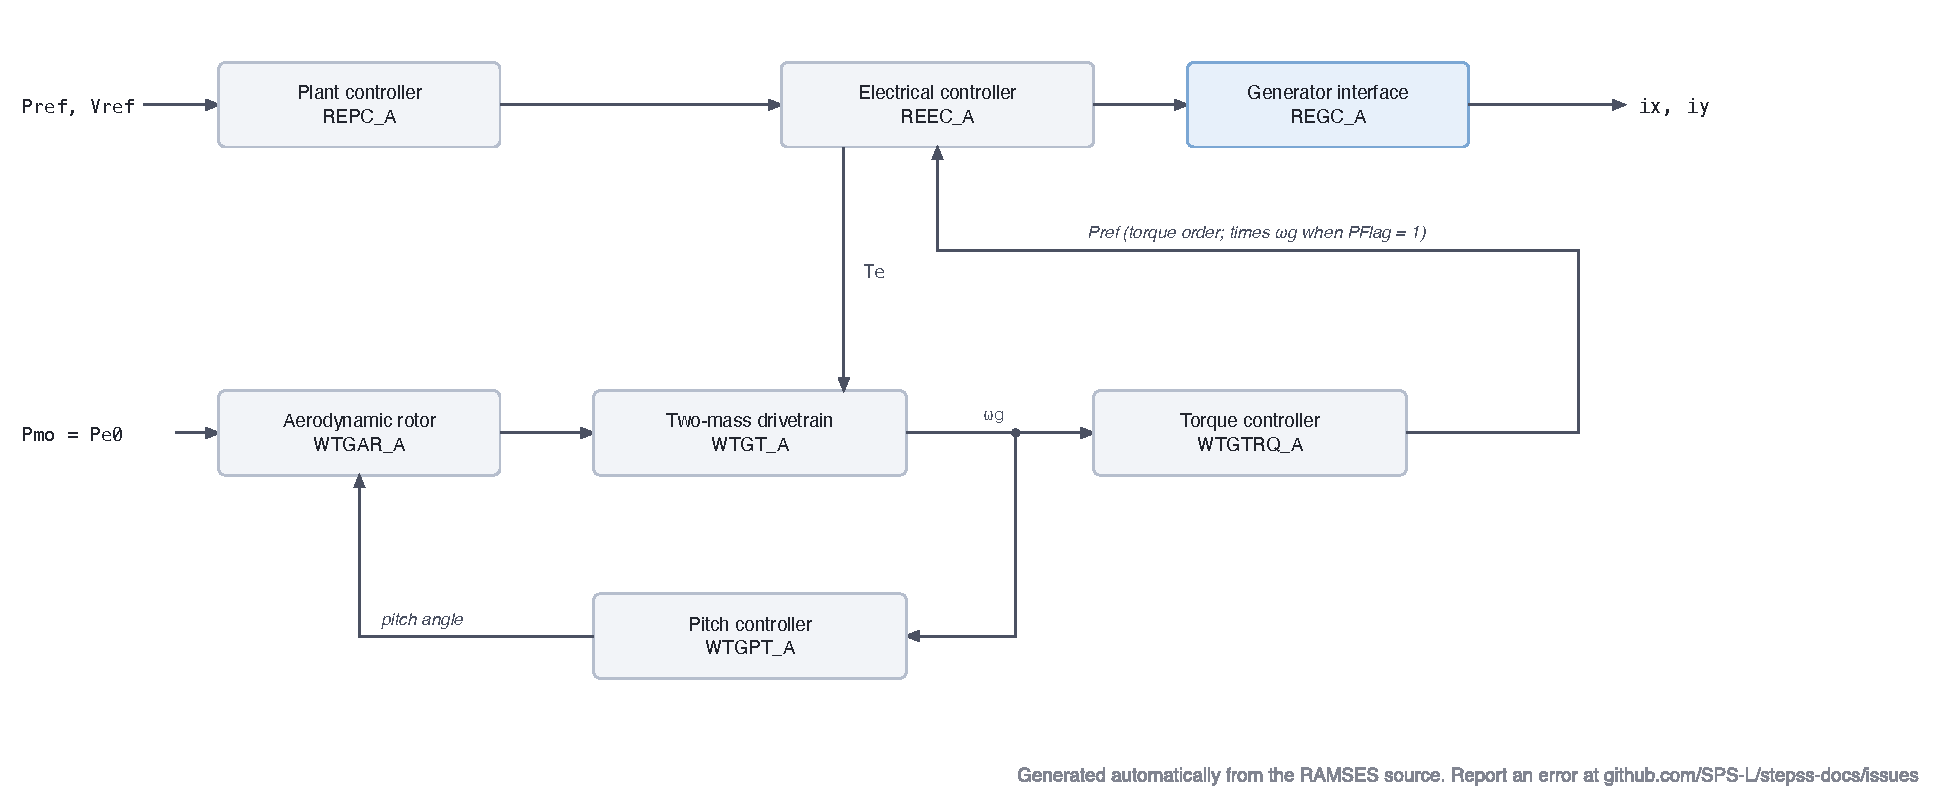
\includegraphics[width=0.98\linewidth]{figures/inj-wt3-light}
\caption{WT3 block diagram.}
\end{figure}

\subsection{Scientific Description}\label{model-inj-wecc:scientific-description}

The equations below are those coded in RAMSES. A flag ``= 1'' is tested in the dynamics as flag \(\geq 0.5\), but initialization tests for exactly 1, so give every flag as exactly \texttt{0} or \texttt{1}.

\textbf{Measurements.} With \(v_t = |\bar V|\) the terminal voltage:

\[P_e = (v_x i_x + v_y i_y)\frac{S_{\mathrm{base}}}{S_{\mathrm{nom}}}, \qquad Q_{\mathrm{gen}} = (v_y i_x - v_x i_y)\frac{S_{\mathrm{base}}}{S_{\mathrm{nom}}}\]

\textbf{REPC\_A, plant controller: voltage or reactive power.} The regulated point is the terminal, shifted by a compensation impedance: \(\bar v_{\mathrm{con}} = \bar V - (R_c + jX_c)\bar I\), and \(P_{\mathrm{branch}}\), \(Q_{\mathrm{branch}}\) are the powers through that point. The measured quantity is

\[Y_1 = \begin{cases} |\bar v_{\mathrm{con}}| & \text{vcompFlag} = 1 \\ v_t + K_c\,Q_{\mathrm{branch}} & \text{vcompFlag} = 0 \end{cases}\]

filtered by \(1/(1+sT_{\mathrm{fltr}})\). The error is \(v_{\mathrm{ref}} - Y_2\) when RefFlag = 1 and \(Q_{\mathrm{ref}} - Q_{\mathrm{branch}}/(1+sT_{\mathrm{fltr}})\) when RefFlag = 0. It passes a symmetric deadband \(\pm\)\texttt{dbd}, the limits {[}\texttt{emin}, \texttt{emax}{]}, and a PI controller (\texttt{Kp}, \texttt{Ki}) whose integrator and output are both limited to {[}\texttt{Qmin}, \texttt{Qmax}{]}. The integrator is frozen while \(v_t <\) \texttt{vfrz}. A lead-lag \((1+sT_{ft})/(1+sT_{fv})\) follows; with \(T_{fv} < 0.005\) s it is bypassed. Its output becomes the reactive power reference \(Q_{\mathrm{ext}}\) of REEC\_A only when QextFlag = 1; with QextFlag = 0, \(Q_{\mathrm{ext}}\) stays at its initial value.

\textbf{REPC\_A, plant controller: frequency.} The bus frequency is estimated from the rotation of the voltage phasor filtered with \(T_m = \max(0.05, T_{\mathrm{mesf}})\):

\[f = \frac{(v_y - v_{yf})\,v_{xf} - (v_x - v_{xf})\,v_{yf}}{2\pi f_{\mathrm{nom}}\, T_m\,(v_{xf}^2 + v_{yf}^2)} + \omega_{\mathrm{ref}}\]

where \(\omega_{\mathrm{ref}}\) is 1 or the centre-of-inertia speed, following \texttt{\$OMEGA\_REF}. The frequency error \(\Delta f = 1 - f\) passes the deadband {[}\texttt{fdbd1}, \texttt{fdbd2}{]} and the droops:

\[e_P = P_{\mathrm{plantref}} - \frac{P_{\mathrm{branch}}}{1+sT_p} + \min(D_{dn}\Delta f, 0) + \max(D_{up}\Delta f, 0)\]

so \texttt{Ddn} acts on over-frequency and \texttt{Dup} on under-frequency. \(e_P\) is limited to {[}\texttt{femin}, \texttt{femax}{]} and fed to a PI (\texttt{kpg}, \texttt{kig}) limited to {[}\texttt{Pmin}, \texttt{Pmax}{]}, then a lag \(1/(1+sT_{\mathrm{lag}})\). The result replaces the active power reference \(P_{\mathrm{refo}}\) only when FreqFlag = 1.

\textbf{WTGTRQ\_A, torque controller.} The electrical power is filtered, \(x_{27} = P_e/(1+sT_p)\), and a piecewise-linear table through (\texttt{p1}, \texttt{spd1}) \ldots{} (\texttt{p4}, \texttt{spd4}), flat outside its end points, gives the speed reference:

\[\omega_{\mathrm{ref}} = \frac{f_{\mathrm{spd}}(x_{27})}{1 + sT_{\mathrm{wref}}}\]

The error is \((P_{\mathrm{refo}} - x_{27})/\omega_g\) when Tflag = 1 (power error) and \(\omega_g - \omega_{\mathrm{ref}}\) when Tflag = 0 (speed error). A PI (\texttt{Kpp}, \texttt{Kip}), integrator and output limited to {[}\texttt{Temin}, \texttt{Temax}{]}, gives the torque order \(P_{\mathrm{ref}}\). The integrator is frozen during a voltage dip.

\textbf{WTGPT\_A, pitch controller.} Two PI controllers, each limited to {[}\texttt{ThetaMin}, \texttt{ThetaMax}{]}, act on the speed error and on the power error:

\[e_\omega = \omega_t - \omega_{\mathrm{ref}} + K_{cc}(P_{\mathrm{ord}} - P_{\mathrm{refo}}), \qquad e_P = P_{\mathrm{ord}} - P_{\mathrm{refo}}\]

(\texttt{Kpw}, \texttt{Kiw}) on \(e_\omega\) and (\texttt{Kpc}, \texttt{Kic}) on \(e_P\). Their sum drives the actuator lag \(1/(1+sT_\theta)\), with the rate limited to {[}\texttt{dThetaMin}, \texttt{dThetaMax}{]} and the angle to {[}\texttt{ThetaMin}, \texttt{ThetaMax}{]}.

\textbf{WTGAR\_A, aerodynamics.}

\[P_m = P_{mo} - K_a\,\theta\,(\theta - \theta_0), \qquad P_{mo} = P_{e0}\]

The pitch angle unit is whatever the data uses, conventionally degrees; \texttt{Ka} must be given per that unit squared.

\textbf{WTGT\_A, two-mass drivetrain.} With \(T_m = P_m/\omega_t\) and \(T_e = P_e/\omega_g\):

\[2H_t\frac{d\Delta\omega_t}{dt} = T_m - K_{\mathrm{shaft}}\Delta\theta - D_{\mathrm{shaft}}(\Delta\omega_t - \Delta\omega_g)\]

\[2H_g\frac{d\Delta\omega_g}{dt} = K_{\mathrm{shaft}}\Delta\theta + D_{\mathrm{shaft}}(\Delta\omega_t - \Delta\omega_g) - T_e\]

\[\frac{d\Delta\theta}{dt} = \Delta\omega_t - \Delta\omega_g, \qquad \omega_t = \omega_o + \Delta\omega_t, \quad \omega_g = \omega_o + \Delta\omega_g\]

The twist equation carries no base angular frequency, so \(\Delta\theta\) is in pu\ensuremath{\cdot}s and \texttt{Kshaft} in pu torque per pu\ensuremath{\cdot}s. A stiffness quoted per electrical radian must be multiplied by \(2\pi f_{\mathrm{nom}}\). The initial speed \(\omega_o\) is read off the power-speed table at \(P_{e0}\), so it is generally not 1.

\textbf{REEC\_A, electrical controller: voltage dip.} A dip is declared when the unfiltered \(v_t <\) \texttt{vdip} or \(v_t >\) \texttt{vup}. During a dip the integrators of the Q, V and torque PIs, the \texttt{Tiq} lag and the power order lag are frozen, and the reactive current injection

\[I_{q,\mathrm{inj}} = \mathrm{lim}_{[I_{ql1},\, I_{qh1}]}\Big(k_{qv}\,\mathrm{db}_{[dbd1,\, dbd2]}\big(v_{\mathrm{ref0}} - v_{t,\mathrm{filt}}\big)\Big)\]

is added to the reactive current command, with \(v_{t,\mathrm{filt}} = v_t/(1+sT_{rv})\). After the dip ends, \texttt{Thld} selects what happens for \(|\)\texttt{Thld}\(|\) seconds: with \texttt{Thld} \(> 0\), \(I_{q,\mathrm{inj}}\) is held at \texttt{Iqfrz}; with \texttt{Thld} \(< 0\), the injection law above stays active; with \texttt{Thld} \(= 0\), \(I_{q,\mathrm{inj}}\) returns to zero at once. The active current limit \(I_{p\max}\) is frozen during the dip and for \texttt{Thld2} seconds after it.

\textbf{REEC\_A, reactive power chain.} The reactive power reference is

\[Q_r = \mathrm{lim}_{[q_{\min},\, q_{\max}]}\begin{cases} x_{27}\tan(\mathrm{pfaref}) & \text{PFFlag} = 1 \text{ (constant power factor)} \\ Q_{\mathrm{ext}} & \text{PFFlag} = 0 \end{cases}\]

With QFlag = 0 the reactive current command is \(\big(Q_r/v_{t,\mathrm{filt}}\big)/(1+sT_{iq})\). With QFlag = 1 it is the output of a voltage PI (\texttt{kvp}, \texttt{kvi}) on \(V_{\mathrm{ref}} - v_{t,\mathrm{filt}}\), limited to {[}\(I_{q\min}\), \(I_{q\max}\){]}, where

\[V_{\mathrm{ref}} = \mathrm{lim}_{[v_{\min},\, v_{\max}]}\begin{cases} \text{Q PI } (k_{qp}, k_{qi}) \text{ on } Q_r - Q_{\mathrm{gen}} & \text{vFlag} = 1 \\ Q_r + v_{\mathrm{ref1}} & \text{vFlag} = 0 \end{cases}\]

In both cases \(I_{q\mathrm{cmd}} = \mathrm{lim}_{[I_{q\min},\, I_{q\max}]}(I_{q,\mathrm{inj}} + \cdots)\).

\textbf{REEC\_A, active power chain.} \(P_{\mathrm{ref}}\) is rate-limited to {[}\texttt{dPmin}, \texttt{dPmax}{]} (per second). With PFlag = 1 it is multiplied by \(\omega_g\), which makes \(P_{\mathrm{ref}}\) a torque and lets drivetrain oscillations reach the output. Then

\[T_{\mathrm{pord}}\frac{dP_{\mathrm{ord}}}{dt} = P_{\mathrm{ref}}\,\omega_g^{\,\mathrm{PFlag}} - P_{\mathrm{ord}}, \quad P_{\mathrm{ord}} \in [p_{\min}, p_{\max}], \qquad I_{p\mathrm{cmd}} = \mathrm{lim}_{[0,\, I_{p\max}]}\frac{P_{\mathrm{ord}}}{\max(v_{t,\mathrm{filt}}, 0.01)}\]

\textbf{REEC\_A, current limits.} \texttt{VDL1} (\texttt{vq1}\ldots{}\texttt{Iq4}) and \texttt{VDL2} (\texttt{vp1}\ldots{}\texttt{Ip4}) are piecewise-linear functions of \(v_{t,\mathrm{filt}}\), flat beyond their end points. With \(I_{q\min} = -I_{q\max}\):

\begin{small}\begin{longtable}[]{@{}
  >{\raggedright\arraybackslash}p{(\linewidth - 6\tabcolsep) * \real{0.3103}}
  >{\raggedright\arraybackslash}p{(\linewidth - 6\tabcolsep) * \real{0.3449}}
  >{\raggedright\arraybackslash}p{(\linewidth - 6\tabcolsep) * \real{0.3449}}
@{}}
\toprule\noalign{}
\begin{minipage}[b]{\linewidth}\raggedright
PQFlag
\end{minipage} & \begin{minipage}[b]{\linewidth}\raggedright
\(I_{q\max}\)
\end{minipage} & \begin{minipage}[b]{\linewidth}\raggedright
\(I_{p\max}\)
\end{minipage} \\
\midrule\noalign{}
\endhead
\bottomrule\noalign{}
\endlastfoot
0 (Q priority) & \(\min(\mathrm{VDL1}, I_{\max})\) & \(\min\big(\mathrm{VDL2}, \sqrt{I_{\max}^2 - I_{q\mathrm{cmd}}^2}\big)\) \\
1 (P priority) & \(\min\big(\mathrm{VDL1}, \sqrt{I_{\max}^2 - I_{p\mathrm{cmd}}^2}\big)\) & \(\min(\mathrm{VDL2}, I_{\max})\) \\
\end{longtable}\end{small}

\textbf{REGC\_A, generator/converter.} Both current commands pass a lag of time constant \texttt{Tg}. The rate of the reactive current is limited in one direction only, chosen from the sign of the initial reactive power: by \texttt{Iqrmax} if \(Q_0 > 0\), by \texttt{Iqrmin} if \(Q_0 < 0\), not at all if \(Q_0 = 0\). The rise of the active current is limited to \texttt{rrpwr} per second at all times. High-voltage reactive current management and low-voltage active current management then give the injected currents:

\[I_{qf} = \frac{\max\big(I_q v_t - \max(0,\, K_{hv}(v_t - V_{olim})),\ \text{QMIN}\big)}{v_t/(1+sT_{\mathrm{fltr}})}, \qquad I_{pf} = m(v_t)\, I_p\]

where \(K_{hv}\) is \texttt{accel}, \(V_{olim}\) is \texttt{vtmax}, and \(m\) rises linearly from 0 at \texttt{lvpnt0} to 1 at \texttt{lvpnt1}. When \texttt{Lvplsw} = 1, \(I_p\) is also capped by the low-voltage power logic: zero below \texttt{zerox}, rising linearly to \texttt{Lvpl1} at \texttt{Brkpt}, no cap above \texttt{Brkpt}. The voltage it uses is \(v_t/(1+sT_{\mathrm{fltr}})\).

\textbf{PLL.} The voltage components are filtered with \(T_{\mathrm{fltr}}\) and

\[v_q = -v_{xf}\sin\theta_{\mathrm{pll}} + v_{yf}\cos\theta_{\mathrm{pll}}, \qquad \omega_{\mathrm{pll}} = k_{p,\mathrm{PLL}}\,v_q + k_{i,\mathrm{PLL}}\!\int v_q\,dt, \qquad \frac{d\theta_{\mathrm{pll}}}{dt} = \omega_{\mathrm{pll}} - \omega_{\mathrm{ref,PLL}}\]

The angle is frozen while the filtered voltage is below \texttt{vPLL}. The angle equation carries no base angular frequency, so \texttt{kpPLL} and \texttt{kiPLL} are in rad/s per pu. \texttt{wrefPLL} is also the initial value of \(\omega_{\mathrm{pll}}\), so it cancels and has no effect on the response.

\textbf{Network interface.} The injected current is resolved with the PLL angle and rescaled to the system base:

\[i_x = \left(I_{pf}\cos\theta_{\mathrm{pll}} + I_{qf}\sin\theta_{\mathrm{pll}}\right)\frac{S_{\mathrm{nom}}}{S_{\mathrm{base}}}, \qquad i_y = \left(I_{pf}\sin\theta_{\mathrm{pll}} - I_{qf}\cos\theta_{\mathrm{pll}}\right)\frac{S_{\mathrm{nom}}}{S_{\mathrm{base}}}\]

A positive \(I_{qf}\) injects reactive power. \hyperref[model-inj-wecc:wt4-inj_wt4-type-4-wind-turbine-full-converter]{WT4} and \hyperref[model-inj-wecc:bess-inj_bess-battery-energy-storage-system]{BESS} use the same interface.

\textbf{Reactive power control modes.} The flags combine as in the WECC specification:

\begin{small}\begin{longtable}[]{@{}llllll@{}}
\toprule\noalign{}
Mode & PFFlag & vFlag & QFlag & RefFlag & QextFlag \\
\midrule\noalign{}
\endhead
\bottomrule\noalign{}
\endlastfoot
Constant power factor & 1 & any & 0 & any & 0 \\
Constant Q & 0 & any & 0 & any & 0 \\
Local voltage control & 0 & 0 & 1 & any & 0 \\
Local coordinated Q/V control & 0 & 1 & 1 & any & 0 \\
Plant Q control & 0 & any & 0 & 0 & 1 \\
Plant voltage control & 0 & any & 0 & 1 & 1 \\
Plant voltage control + local coordinated Q/V & 0 & 1 & 1 & 1 & 1 \\
Plant Q control + local coordinated Q/V & 0 & 1 & 1 & 0 & 1 \\
\end{longtable}\end{small}

\subsection{Parameters}\label{model-inj-wecc:parameters}

RAMSES applies \textbf{no default values}: a \texttt{WT3} record must carry exactly 128 values, and one with more or fewer is refused. The \emph{Example} column is the record in the usage example below. Per-unit values are on \texttt{SNOM} unless stated. The REPC\_A, REEC\_A, REGC\_A and PLL blocks are the same code in WT4 at the indices given in the \emph{WT4 \#} column.

\textbf{Rating and REPC\_A plant controller}

\begin{small}\begin{longtable}[]{@{}
  >{\raggedright\arraybackslash}p{(\linewidth - 12\tabcolsep) * \real{0.0939}}
  >{\raggedright\arraybackslash}p{(\linewidth - 12\tabcolsep) * \real{0.0939}}
  >{\raggedright\arraybackslash}p{(\linewidth - 12\tabcolsep) * \real{0.1408}}
  >{\raggedright\arraybackslash}p{(\linewidth - 12\tabcolsep) * \real{0.4391}}
  >{\raggedright\arraybackslash}p{(\linewidth - 12\tabcolsep) * \real{0.1149}}
  >{\raggedright\arraybackslash}p{(\linewidth - 12\tabcolsep) * \real{0.1175}}
@{}}
\toprule\noalign{}
\begin{minipage}[b]{\linewidth}\raggedright
WT3 \#
\end{minipage} & \begin{minipage}[b]{\linewidth}\raggedright
WT4 \#
\end{minipage} & \begin{minipage}[b]{\linewidth}\raggedright
Name
\end{minipage} & \begin{minipage}[b]{\linewidth}\raggedright
Description
\end{minipage} & \begin{minipage}[b]{\linewidth}\raggedright
Unit
\end{minipage} & \begin{minipage}[b]{\linewidth}\raggedright
Example
\end{minipage} \\
\midrule\noalign{}
\endhead
\bottomrule\noalign{}
\endlastfoot
1 & 1 & \texttt{SNOM} & Rating, base of every per-unit quantity in the model & MVA & 1.667 \\
2 & 2 & \texttt{Rc} & Compensation resistance & pu & 0 \\
3 & 3 & \texttt{Xc} & Compensation reactance (droop or line-drop) & pu & 0 \\
4 & 4 & \texttt{vcompFlag} & 1: regulate \(\lvert\bar v_{\mathrm{con}}\rvert\) (line-drop compensation); 0: regulate \(v_t + K_c Q_{\mathrm{branch}}\) (droop) & & 0 \\
5 & 5 & \texttt{Kc} & Reactive droop gain (used when \texttt{vcompFlag} = 0) & pu/pu & 0 \\
6 & 6 & \texttt{Tfltr} & Voltage and Q measurement filter; also the REGC\_A voltage filter and the PLL input filter & s & 0.02 \\
7 & 7 & \texttt{RefFlag} & 1: voltage control; 0: reactive power control & & 1 \\
8 & 8 & \texttt{dbd} & Deadband on the V/Q error, symmetric, \(\geq 0\) & pu & 0 \\
9 & 9 & \texttt{emax} & Upper limit on the V/Q error & pu & 0.1 \\
10 & 10 & \texttt{emin} & Lower limit on the V/Q error & pu & -0.1 \\
11 & 11 & \texttt{Kp} & V/Q PI proportional gain & pu/pu & 18 \\
12 & 12 & \texttt{Ki} & V/Q PI integral gain & pu/(pu\ensuremath{\cdot}s) & 5 \\
13 & 13 & \texttt{Qmax} & Upper limit of the V/Q PI & pu & 0.44 \\
14 & 14 & \texttt{Qmin} & Lower limit of the V/Q PI & pu & -0.44 \\
15 & 15 & \texttt{Tft} & Lead time constant & s & 0 \\
16 & 16 & \texttt{Tfv} & Lag time constant; below 0.005 the lead-lag is bypassed & s & 0.05 \\
17 & 17 & \texttt{vfrz} & Voltage below which the V/Q integrator is frozen & pu & 0.7 \\
18 & 18 & \texttt{Tp} & Filter on \(P_{\mathrm{branch}}\); also the \(P_e\) filter of WTGTRQ\_A (WT3) and of the power-factor reference & s & 0.05 \\
19 & 19 & \texttt{fdbd1} & Frequency deadband, lower edge, \(\leq 0\) & pu & -0.0006 \\
20 & 20 & \texttt{fdbd2} & Frequency deadband, upper edge, \(\geq 0\) & pu & 0.0006 \\
21 & 21 & \texttt{Ddn} & Droop for over-frequency & pu/pu & 20 \\
22 & 22 & \texttt{Dup} & Droop for under-frequency & pu/pu & 0 \\
23 & 23 & \texttt{femax} & Upper limit on the power error & pu & 999 \\
24 & 24 & \texttt{femin} & Lower limit on the power error & pu & -999 \\
25 & 25 & \texttt{kpg} & Power PI proportional gain & pu/pu & 0.05 \\
26 & 26 & \texttt{kig} & Power PI integral gain & pu/(pu\ensuremath{\cdot}s) & 0.1 \\
27 & 27 & \texttt{Pmax} & Upper limit of the power PI & pu & 1 \\
28 & 28 & \texttt{Pmin} & Lower limit of the power PI & pu & 0 \\
29 & 29 & \texttt{Tlag} & Lag on the plant power output & s & 0.1 \\
30 & 30 & \texttt{FreqFlag} & 1: plant power loop sets \(P_{\mathrm{refo}}\); 0: \(P_{\mathrm{refo}}\) held at its initial value & & 0 \\
31 & 31 & \texttt{Tmesf} & Frequency measurement time constant, raised to 0.05 if smaller & s & 0.02 \\
32 & 32 & \texttt{QextFlag} & 1: plant V/Q loop sets \(Q_{\mathrm{ext}}\); 0: \(Q_{\mathrm{ext}}\) held at its initial value & & 0 \\
\end{longtable}\end{small}

With \texttt{FreqFlag} = 0 and \texttt{QextFlag} = 0, as in the example, REPC\_A is computed but drives nothing.

\textbf{WTGTRQ\_A torque controller} (WT3 only)

\begin{small}\begin{longtable}[]{@{}lllll@{}}
\toprule\noalign{}
WT3 \# & Name & Description & Unit & Example \\
\midrule\noalign{}
\endhead
\bottomrule\noalign{}
\endlastfoot
33 & \texttt{Twref} & Speed reference time constant & s & 30 \\
34 & \texttt{Kip} & Torque PI integral gain & pu/(pu\ensuremath{\cdot}s) & 0.6 \\
35 & \texttt{Kpp} & Torque PI proportional gain & pu/pu & 3 \\
36 & \texttt{Temax} & Maximum torque order & pu & 1.2 \\
37 & \texttt{Temin} & Minimum torque order & pu & 0 \\
38 & \texttt{p1} & Power-speed table, power of point 1 & pu & 0.2 \\
39 & \texttt{spd1} & Power-speed table, speed of point 1 & pu & 0.58 \\
40 & \texttt{p2} & Point 2, power & pu & 0.4 \\
41 & \texttt{spd2} & Point 2, speed & pu & 0.72 \\
42 & \texttt{p3} & Point 3, power & pu & 0.6 \\
43 & \texttt{spd3} & Point 3, speed & pu & 0.86 \\
44 & \texttt{p4} & Point 4, power & pu & 0.8 \\
45 & \texttt{spd4} & Point 4, speed & pu & 1.0 \\
46 & \texttt{Tflag} & 1: PI on power error; 0: PI on speed error & & 1 \\
\end{longtable}\end{small}

\textbf{WTGPT\_A pitch controller} (WT3 only)

\begin{small}\begin{longtable}[]{@{}
  >{\raggedright\arraybackslash}p{(\linewidth - 10\tabcolsep) * \real{0.1138}}
  >{\raggedright\arraybackslash}p{(\linewidth - 10\tabcolsep) * \real{0.1748}}
  >{\raggedright\arraybackslash}p{(\linewidth - 10\tabcolsep) * \real{0.4154}}
  >{\raggedright\arraybackslash}p{(\linewidth - 10\tabcolsep) * \real{0.1734}}
  >{\raggedright\arraybackslash}p{(\linewidth - 10\tabcolsep) * \real{0.1226}}
@{}}
\toprule\noalign{}
\begin{minipage}[b]{\linewidth}\raggedright
WT3 \#
\end{minipage} & \begin{minipage}[b]{\linewidth}\raggedright
Name
\end{minipage} & \begin{minipage}[b]{\linewidth}\raggedright
Description
\end{minipage} & \begin{minipage}[b]{\linewidth}\raggedright
Unit
\end{minipage} & \begin{minipage}[b]{\linewidth}\raggedright
Example
\end{minipage} \\
\midrule\noalign{}
\endhead
\bottomrule\noalign{}
\endlastfoot
47 & \texttt{Kcc} & Gain of the power error added to the speed error & pu/pu & 0 \\
48 & \texttt{Kiw} & Pitch control integral gain & deg/(pu\ensuremath{\cdot}s) & 0.6 \\
49 & \texttt{Kpw} & Pitch control proportional gain & deg/pu & 0.3 \\
50 & \texttt{ThetaMin} & Minimum pitch angle (also limits both PIs) & deg & 0 \\
51 & \texttt{ThetaMax} & Maximum pitch angle (also limits both PIs) & deg & 27 \\
52 & \texttt{Ttheta} & Pitch actuator time constant & s & 0.3 \\
53 & \texttt{Kic} & Pitch compensation integral gain & deg/(pu\ensuremath{\cdot}s) & 0.6 \\
54 & \texttt{Kpc} & Pitch compensation proportional gain & deg/pu & 3 \\
55 & \texttt{dThetaMin} & Minimum pitch rate & deg/s & -10 \\
56 & \texttt{dThetaMax} & Maximum pitch rate & deg/s & 10 \\
\end{longtable}\end{small}

\textbf{WTGAR\_A aerodynamics and WTGT\_A drivetrain} (WT3 only; WT4 has its own drivetrain block, listed under \hyperref[model-inj-wecc:wt4-inj_wt4-type-4-wind-turbine-full-converter]{WT4})

\begin{small}\begin{longtable}[]{@{}lllll@{}}
\toprule\noalign{}
WT3 \# & Name & Description & Unit & Example \\
\midrule\noalign{}
\endhead
\bottomrule\noalign{}
\endlastfoot
57 & \texttt{Ka} & Aerodynamic gain & pu/deg\ensuremath{^2} & 0.007 \\
58 & \texttt{Thetao} & Initial pitch angle \(\theta_0\) & deg & 0 \\
59 & \texttt{Ht} & Turbine inertia & s & 3.395 \\
60 & \texttt{Hg} & Generator inertia & s & 0.962 \\
61 & \texttt{Dshaft} & Shaft damping & pu/pu & 2.344 \\
62 & \texttt{Kshaft} & Shaft stiffness, per pu\ensuremath{\cdot}s of twist & pu & 1.387 \\
\end{longtable}\end{small}

\textbf{REEC\_A electrical controller}

\begin{small}\begin{longtable}[]{@{}
  >{\raggedright\arraybackslash}p{(\linewidth - 12\tabcolsep) * \real{0.1136}}
  >{\raggedright\arraybackslash}p{(\linewidth - 12\tabcolsep) * \real{0.1075}}
  >{\raggedright\arraybackslash}p{(\linewidth - 12\tabcolsep) * \real{0.1461}}
  >{\raggedright\arraybackslash}p{(\linewidth - 12\tabcolsep) * \real{0.3945}}
  >{\raggedright\arraybackslash}p{(\linewidth - 12\tabcolsep) * \real{0.1236}}
  >{\raggedright\arraybackslash}p{(\linewidth - 12\tabcolsep) * \real{0.1146}}
@{}}
\toprule\noalign{}
\begin{minipage}[b]{\linewidth}\raggedright
WT3 \#
\end{minipage} & \begin{minipage}[b]{\linewidth}\raggedright
WT4 \#
\end{minipage} & \begin{minipage}[b]{\linewidth}\raggedright
Name
\end{minipage} & \begin{minipage}[b]{\linewidth}\raggedright
Description
\end{minipage} & \begin{minipage}[b]{\linewidth}\raggedright
Unit
\end{minipage} & \begin{minipage}[b]{\linewidth}\raggedright
Example
\end{minipage} \\
\midrule\noalign{}
\endhead
\bottomrule\noalign{}
\endlastfoot
63 & 38 & \texttt{vdip} & Voltage below which a dip is declared & pu & 0.9 \\
64 & 39 & \texttt{vup} & Voltage above which a dip is declared & pu & 1.1 \\
65 & 40 & \texttt{Trv} & Terminal voltage filter & s & 0.02 \\
66 & 41 & \texttt{vref0} & Reference for the dip injection; used as given, so 0 is not replaced by the initial voltage & pu & 1 \\
67 & 42 & \texttt{vref1} & Bias added to \(Q_r\) when vFlag = 0 & pu & 1 \\
68 & 43 & \texttt{dbd1} & Dip injection deadband, lower edge, \(\leq 0\) & pu & -0.05 \\
69 & 44 & \texttt{dbd2} & Dip injection deadband, upper edge, \(\geq 0\) & pu & 0.05 \\
70 & 45 & \texttt{kqv} & Dip reactive current gain & pu/pu & 2 \\
71 & 46 & \texttt{Iqh1} & Upper limit of the dip injection & pu & 1.05 \\
72 & 47 & \texttt{Iql1} & Lower limit of the dip injection & pu & -1.05 \\
73 & 48 & \texttt{qmax} & Upper limit of \(Q_r\) & pu & 0.44 \\
74 & 49 & \texttt{qmin} & Lower limit of \(Q_r\) & pu & -0.44 \\
75 & 50 & \texttt{vmax} & Upper limit of \(V_{\mathrm{ref}}\) and of the Q PI & pu & 1.1 \\
76 & 51 & \texttt{vmin} & Lower limit of \(V_{\mathrm{ref}}\) and of the Q PI & pu & 0.9 \\
77 & 52 & \texttt{kqp} & Q PI proportional gain & pu/pu & 0 \\
78 & 53 & \texttt{kqi} & Q PI integral gain & pu/(pu\ensuremath{\cdot}s) & 0.1 \\
79 & 54 & \texttt{kvp} & V PI proportional gain & pu/pu & 0 \\
80 & 55 & \texttt{kvi} & V PI integral gain & pu/(pu\ensuremath{\cdot}s) & 40 \\
81 & 56 & \texttt{Tiq} & Reactive current lag (QFlag = 0) & s & 0.02 \\
82 & 57 & \texttt{vq1} & VDL1, voltage of point 1 & pu & 0.2 \\
83 & 58 & \texttt{Iq1} & VDL1, reactive current limit at point 1 & pu & 1 \\
84 & 59 & \texttt{vq2} & VDL1, point 2 & pu & 0.4 \\
85 & 60 & \texttt{Iq2} & & pu & 1 \\
86 & 61 & \texttt{vq3} & VDL1, point 3 & pu & 0.8 \\
87 & 62 & \texttt{Iq3} & & pu & 1 \\
88 & 63 & \texttt{vq4} & VDL1, point 4 & pu & 1 \\
89 & 64 & \texttt{Iq4} & & pu & 1 \\
90 & 65 & \texttt{vp1} & VDL2, voltage of point 1 & pu & 0.2 \\
91 & 66 & \texttt{Ip1} & VDL2, active current limit at point 1 & pu & 1 \\
92 & 67 & \texttt{vp2} & VDL2, point 2 & pu & 0.4 \\
93 & 68 & \texttt{Ip2} & & pu & 1 \\
94 & 69 & \texttt{vp3} & VDL2, point 3 & pu & 0.8 \\
95 & 70 & \texttt{Ip3} & & pu & 1 \\
96 & 71 & \texttt{vp4} & VDL2, point 4 & pu & 1 \\
97 & 72 & \texttt{Ip4} & & pu & 1 \\
98 & 73 & \texttt{dPmax} & Upper rate limit of \(P_{\mathrm{ref}}\) & pu/s & 999 \\
99 & 74 & \texttt{dPmin} & Lower rate limit of \(P_{\mathrm{ref}}\) & pu/s & -999 \\
100 & 75 & \texttt{pmax} & Upper limit of \(P_{\mathrm{ord}}\) & pu & 1 \\
101 & 76 & \texttt{pmin} & Lower limit of \(P_{\mathrm{ord}}\) & pu & 0 \\
102 & 77 & \texttt{Tpord} & Power order lag & s & 0.02 \\
103 & 78 & \texttt{Imax} & Converter current limit & pu & 1.11 \\
104 & 79 & \texttt{Thld} & Post-dip hold of the reactive injection; its sign selects the mode & s & 0 \\
105 & 80 & \texttt{Thld2} & Post-dip hold of \(I_{p\max}\) & s & 0 \\
106 & 81 & \texttt{Iqfrz} & Reactive injection held after a dip when \texttt{Thld} \(> 0\) & pu & 0 \\
107 & 82 & \texttt{PFFlag} & 1: constant power factor; 0: reactive power reference \(Q_{\mathrm{ext}}\) & & 0 \\
108 & 83 & \texttt{vFlag} & 1: \(V_{\mathrm{ref}}\) from the Q PI; 0: \(V_{\mathrm{ref}} = Q_r + v_{\mathrm{ref1}}\) & & 0 \\
109 & 84 & \texttt{QFlag} & 1: reactive current from the voltage PI; 0: from \(Q_r/v_t\) & & 0 \\
110 & 85 & \texttt{PQFlag} & 1: active current priority; 0: reactive current priority & & 0 \\
111 & 86 & \texttt{PFlag} & 1: power order is \(P_{\mathrm{ref}}\,\omega_g\); 0: power order is \(P_{\mathrm{ref}}\) & & 1 \\
\end{longtable}\end{small}

\textbf{REGC\_A generator/converter and PLL}

\begin{small}\begin{longtable}[]{@{}
  >{\raggedright\arraybackslash}p{(\linewidth - 12\tabcolsep) * \real{0.1164}}
  >{\raggedright\arraybackslash}p{(\linewidth - 12\tabcolsep) * \real{0.1020}}
  >{\raggedright\arraybackslash}p{(\linewidth - 12\tabcolsep) * \real{0.1484}}
  >{\raggedright\arraybackslash}p{(\linewidth - 12\tabcolsep) * \real{0.4034}}
  >{\raggedright\arraybackslash}p{(\linewidth - 12\tabcolsep) * \real{0.1154}}
  >{\raggedright\arraybackslash}p{(\linewidth - 12\tabcolsep) * \real{0.1143}}
@{}}
\toprule\noalign{}
\begin{minipage}[b]{\linewidth}\raggedright
WT3 \#
\end{minipage} & \begin{minipage}[b]{\linewidth}\raggedright
WT4 \#
\end{minipage} & \begin{minipage}[b]{\linewidth}\raggedright
Name
\end{minipage} & \begin{minipage}[b]{\linewidth}\raggedright
Description
\end{minipage} & \begin{minipage}[b]{\linewidth}\raggedright
Unit
\end{minipage} & \begin{minipage}[b]{\linewidth}\raggedright
Example
\end{minipage} \\
\midrule\noalign{}
\endhead
\bottomrule\noalign{}
\endlastfoot
112 & 87 & \texttt{Iqrmax} & Reactive current rate limit, used when \(Q_0 > 0\) & pu/s & 999 \\
113 & 88 & \texttt{Iqrmin} & Reactive current rate limit, used when \(Q_0 < 0\) & pu/s & -999 \\
114 & 89 & \texttt{Tg} & Converter current lag & s & 0.02 \\
115 & 90 & \texttt{vtmax} & High-voltage threshold (WECC \texttt{Volim}) & pu & 1.2 \\
116 & 91 & \texttt{accel} & High-voltage reactive current gain (WECC \texttt{Khv}) & pu/pu & 0.7 \\
117 & 92 & \texttt{QMIN} & Lower limit of \(I_q v_t\) less the high-voltage term (WECC \texttt{Iolim}) & pu & -1.3 \\
118 & 93 & \texttt{lvpnt0} & Active current is zero below this voltage & pu & 0.4 \\
119 & 94 & \texttt{lvpnt1} & Active current is unreduced above this voltage & pu & 0.8 \\
120 & 95 & \texttt{Brkpt} & Low-voltage power logic breakpoint & pu & 0.9 \\
121 & 96 & \texttt{zerox} & Low-voltage power logic zero crossing & pu & 0.4 \\
122 & 97 & \texttt{Lvpl1} & Low-voltage power logic limit at \texttt{Brkpt} & pu & 1.22 \\
123 & 98 & \texttt{Lvplsw} & 1: low-voltage power logic on; 0: off & & 0 \\
124 & 99 & \texttt{rrpwr} & Active current rise rate limit & pu/s & 10 \\
125 & 100 & \texttt{vPLL} & Voltage below which the PLL angle is frozen & pu & 0.2 \\
126 & 101 & \texttt{kpPLL} & PLL proportional gain & rad/s/pu & 3 \\
127 & 102 & \texttt{kiPLL} & PLL integral gain & rad/s\ensuremath{^2}/pu & 30 \\
128 & 103 & \texttt{wrefPLL} & PLL frequency offset; cancels, no effect on the response & & 1 \\
\end{longtable}\end{small}

\textbf{Time constants.} A zero \texttt{Tfltr}, \texttt{Tp}, \texttt{Tlag}, \texttt{Twref} or \texttt{Trv} turns its block into a direct pass-through. \texttt{Ttheta} below 0.001 does the same for the pitch actuator but also removes every pitch limit, including those of the two PIs.

\begin{docsnote}{Caution}

Keep \texttt{Tiq}, \texttt{Tpord} and \texttt{Tg} at 0.005 s or more, and \texttt{Ht} and \texttt{Hg} well above zero. Below that threshold RAMSES switches these blocks to an algebraic form that does not reduce to a pass-through: \texttt{Tiq} and \texttt{Tpord} then give half the intended value, and \texttt{Tg} breaks the active current channel.

\end{docsnote}

Thirty-one further parameters are computed at initialization. Among them are the power-flow quantities \texttt{vto}, \texttt{Peo}, \texttt{Qgeno} and \texttt{pfaref} (the initial power factor angle, rad), the references \texttt{Qextini}, \texttt{Prefini}, \texttt{vref}, \texttt{Qref} and \texttt{Plantpref} held by REPC\_A, and \texttt{wo}, the initial speed read off the power-speed table.

\subsection{Observables}\label{model-inj-wecc:observables}

All quantities are in pu on \texttt{SNOM}.

\begin{small}\begin{longtable}[]{@{}
  >{\raggedright\arraybackslash}p{(\linewidth - 8\tabcolsep) * \real{0.1886}}
  >{\raggedright\arraybackslash}p{(\linewidth - 8\tabcolsep) * \real{0.3105}}
  >{\raggedright\arraybackslash}p{(\linewidth - 8\tabcolsep) * \real{0.1590}}
  >{\raggedright\arraybackslash}p{(\linewidth - 8\tabcolsep) * \real{0.3420}}
@{}}
\toprule\noalign{}
\begin{minipage}[b]{\linewidth}\raggedright
Name
\end{minipage} & \begin{minipage}[b]{\linewidth}\raggedright
Description
\end{minipage} & \begin{minipage}[b]{\linewidth}\raggedright
Name
\end{minipage} & \begin{minipage}[b]{\linewidth}\raggedright
Description
\end{minipage} \\
\midrule\noalign{}
\endhead
\bottomrule\noalign{}
\endlastfoot
\texttt{Pe}, \texttt{Qgen} & Terminal active and reactive power & \texttt{wg}, \texttt{wt} & Generator and turbine speed \\
\texttt{vt} & Terminal voltage & \texttt{wref} & Speed reference \\
\texttt{Freq} & Measured frequency & \texttt{Pref} & Torque order from WTGTRQ\_A \\
\texttt{vcon} & Compensated voltage & \texttt{Pord} & Power order \\
\texttt{Pbranch}, \texttt{Qbranch} & Powers at the compensated point & \texttt{Theta} & Pitch angle (data unit, degrees by convention) \\
\texttt{Prefo}, \texttt{Qext} & Active and reactive references into WTGTRQ\_A and REEC\_A & \texttt{Pm}, \texttt{Tm}, \texttt{Te} & Mechanical power, mechanical and electrical torque \\
\texttt{Plantpref}, \texttt{Qref}, \texttt{vref} & REPC\_A references, constant & \texttt{Iqinj} & Dip reactive current injection \\
\texttt{Ipcmd}, \texttt{Iqcmd} & Current commands & \texttt{Ipmax}, \texttt{Iqmax}, \texttt{Iqmin} & Current limits \\
\texttt{Ipf}, \texttt{Iqf} & Injected currents & \texttt{x59} & Low-voltage power logic limit on \(I_p\); reads \(10^9\) when inactive \\
\end{longtable}\end{small}

\subsection{Initialization}\label{model-inj-wecc:initialization}

The model initializes from the power-flow voltage and injection: the PLL angle from the bus voltage angle, the converter currents by rotation into that frame, then every block backwards to its references. The mechanical side starts with \(P_m = P_e\) and the speed read off the power-speed table.

RAMSES stops the simulation if the initial point violates the current limits or the dip thresholds: \(I_{q\mathrm{cmd}}\) outside \(\pm I_{q\max}\), \(I_{p\mathrm{cmd}}\) outside \([0, I_{p\max}]\) (which also rejects a unit absorbing active power), or \(v_t\) outside {[}\texttt{vdip}, \texttt{vup}{]}. No other limit is checked, so a PI or a lag can start on its limit without a warning. The initial voltage must also exceed \texttt{lvpnt0}.

\subsection{Usage Example}\label{model-inj-wecc:usage-example}

A 1.667 MVA unit taking its whole operating point from the power flow (\texttt{FP} = \texttt{FQ} = 1), with the plant controller disconnected (\texttt{FreqFlag} = \texttt{QextFlag} = 0), constant reactive power and the drivetrain coupled to the output (\texttt{PFlag} = 1). This is the record of the \texttt{3-bus} case in \texttt{stepss-test-systems}. Lines starting with \texttt{\#} inside a record are ignored.

\begin{Verbatim}
INJEC  WT3  DFIGB03  B03
      # FP FQ P Q: share of the power-flow injection (FP, FQ) or initial power (P in MW, Q in Mvar)
      1.  1.  0.  0.
      # SNOM: Rating, base of every per-unit quantity in the model (MVA)
      1.667
      # Rc: Compensation resistance (pu)
      0
      # Xc: Compensation reactance (droop or line-drop) (pu)
      0
      # vcompFlag: 1: regulate lvertbar v_conrvert (line-drop compensation); 0: regulate v_t + K_c Q_branch (droop)
      0
      # Kc: Reactive droop gain (used when vcompFlag = 0) (pu/pu)
      0
      # Tfltr: Voltage and Q measurement filter; also the REGC_A voltage filter and the PLL input filter (s)
      0.02
      # RefFlag: 1: voltage control; 0: reactive power control
      1
      # dbd: Deadband on the V/Q error, symmetric, geq 0 (pu)
      0
      # emax: Upper limit on the V/Q error (pu)
      0.1
      # emin: Lower limit on the V/Q error (pu)
      -0.1
      # Kp: V/Q PI proportional gain (pu/pu)
      18
      # Ki: V/Q PI integral gain (pu/(pu*s))
      5
      # Qmax: Upper limit of the V/Q PI (pu)
      0.44
      # Qmin: Lower limit of the V/Q PI (pu)
      -0.44
      # Tft: Lead time constant (s)
      0
      # Tfv: Lag time constant; below 0.005 the lead-lag is bypassed (s)
      0.05
      # vfrz: Voltage below which the V/Q integrator is frozen (pu)
      0.7
      # Tp: Filter on P_branch; also the P_e filter of WTGTRQ_A (WT3) and of the power-factor reference (s)
      0.05
      # fdbd1: Frequency deadband, lower edge, leq 0 (pu)
      -0.0006
      # fdbd2: Frequency deadband, upper edge, geq 0 (pu)
      0.0006
      # Ddn: Droop for over-frequency (pu/pu)
      20
      # Dup: Droop for under-frequency (pu/pu)
      0
      # femax: Upper limit on the power error (pu)
      999
      # femin: Lower limit on the power error (pu)
      -999
      # kpg: Power PI proportional gain (pu/pu)
      0.05
      # kig: Power PI integral gain (pu/(pu*s))
      0.1
      # Pmax: Upper limit of the power PI (pu)
      1
      # Pmin: Lower limit of the power PI (pu)
      0
      # Tlag: Lag on the plant power output (s)
      0.1
      # FreqFlag: 1: plant power loop sets P_refo; 0: P_refo held at its initial value
      0
      # Tmesf: Frequency measurement time constant, raised to 0.05 if smaller (s)
      0.02
      # QextFlag: 1: plant V/Q loop sets Q_ext; 0: Q_ext held at its initial value
      0
      # Twref: Speed reference time constant (s)
      30
      # Kip: Torque PI integral gain (pu/(pu*s))
      0.6
      # Kpp: Torque PI proportional gain (pu/pu)
      3
      # Temax: Maximum torque order (pu)
      1.2
      # Temin: Minimum torque order (pu)
      0
      # p1: Power-speed table, power of point 1 (pu)
      0.2
      # spd1: Power-speed table, speed of point 1 (pu)
      0.58
      # p2: Point 2, power (pu)
      0.4
      # spd2: Point 2, speed (pu)
      0.72
      # p3: Point 3, power (pu)
      0.6
      # spd3: Point 3, speed (pu)
      0.86
      # p4: Point 4, power (pu)
      0.8
      # spd4: Point 4, speed (pu)
      1
      # Tflag: 1: PI on power error; 0: PI on speed error
      1
      # Kcc: Gain of the power error added to the speed error (pu/pu)
      0
      # Kiw: Pitch control integral gain (deg/(pu*s))
      0.6
      # Kpw: Pitch control proportional gain (deg/pu)
      0.3
      # ThetaMin: Minimum pitch angle (also limits both PIs) (deg)
      0
      # ThetaMax: Maximum pitch angle (also limits both PIs) (deg)
      27
      # Ttheta: Pitch actuator time constant (s)
      0.3
      # Kic: Pitch compensation integral gain (deg/(pu*s))
      0.6
      # Kpc: Pitch compensation proportional gain (deg/pu)
      3
      # dThetaMin: Minimum pitch rate (deg/s)
      -10
      # dThetaMax: Maximum pitch rate (deg/s)
      10
      # Ka: Aerodynamic gain (pu/deg^2)
      0.007
      # Thetao: Initial pitch angle theta_0 (deg)
      0
      # Ht: Turbine inertia (s)
      3.395
      # Hg: Generator inertia (s)
      0.962
      # Dshaft: Shaft damping (pu/pu)
      2.344
      # Kshaft: Shaft stiffness, per pu*s of twist (pu)
      1.387
      # vdip: Voltage below which a dip is declared (pu)
      0.9
      # vup: Voltage above which a dip is declared (pu)
      1.1
      # Trv: Terminal voltage filter (s)
      0.02
      # vref0: Reference for the dip injection; used as given, so 0 is not replaced by the initial voltage (pu)
      1
      # vref1: Bias added to Q_r when vFlag = 0 (pu)
      1
      # dbd1: Dip injection deadband, lower edge, leq 0 (pu)
      -0.05
      # dbd2: Dip injection deadband, upper edge, geq 0 (pu)
      0.05
      # kqv: Dip reactive current gain (pu/pu)
      2
      # Iqh1: Upper limit of the dip injection (pu)
      1.05
      # Iql1: Lower limit of the dip injection (pu)
      -1.05
      # qmax: Upper limit of the reactive power reference (pu)
      0.44
      # qmin: Lower limit of the reactive power reference (pu)
      -0.44
      # vmax: Upper limit of V_ref and of the Q PI (pu)
      1.1
      # vmin: Lower limit of V_ref and of the Q PI (pu)
      0.9
      # kqp: Q PI proportional gain (pu/pu)
      0
      # kqi: Q PI integral gain (pu/(pu*s))
      0.1
      # kvp: V PI proportional gain (pu/pu)
      0
      # kvi: V PI integral gain (pu/(pu*s))
      40
      # Tiq: Reactive current lag (QFlag = 0) (s)
      0.02
      # vq1: VDL1, voltage of point 1 (pu)
      0.2
      # Iq1: VDL1, reactive current limit at point 1 (pu)
      1
      # vq2: VDL1, point 2 (pu)
      0.4
      # Iq2:  (pu)
      1
      # vq3: VDL1, point 3 (pu)
      0.8
      # Iq3:  (pu)
      1
      # vq4: VDL1, point 4 (pu)
      1
      # Iq4:  (pu)
      1
      # vp1: VDL2, voltage of point 1 (pu)
      0.2
      # Ip1: VDL2, active current limit at point 1 (pu)
      1
      # vp2: VDL2, point 2 (pu)
      0.4
      # Ip2:  (pu)
      1
      # vp3: VDL2, point 3 (pu)
      0.8
      # Ip3:  (pu)
      1
      # vp4: VDL2, point 4 (pu)
      1
      # Ip4:  (pu)
      1
      # dPmax: Upper rate limit of P_ref (pu/s)
      999
      # dPmin: Lower rate limit of P_ref (pu/s)
      -999
      # pmax: Upper limit of the power order Pord (pu)
      1
      # pmin: Lower limit of the power order Pord (pu)
      0
      # Tpord: Power order lag (s)
      0.02
      # Imax: Converter current limit (pu)
      1.11
      # Thld: Post-dip hold of the reactive injection; its sign selects the mode (s)
      0
      # Thld2: Post-dip hold of I_pmax (s)
      0
      # Iqfrz: Reactive injection held after a dip when Thld > 0 (pu)
      0
      # PFFlag: 1: constant power factor; 0: reactive power reference Q_ext
      0
      # vFlag: 1: V_ref from the Q PI; 0: V_ref = Q_r + v_ref1
      0
      # QFlag: 1: reactive current from the voltage PI; 0: from Q_r/v_t
      0
      # PQFlag: 1: active current priority; 0: reactive current priority
      0
      # PFlag: 1: power order is P_ref,omega_g; 0: power order is P_ref
      1
      # Iqrmax: Reactive current rate limit, used when Q_0 > 0 (pu/s)
      999
      # Iqrmin: Reactive current rate limit, used when Q_0 < 0 (pu/s)
      -999
      # Tg: Converter current lag (s)
      0.02
      # vtmax: High-voltage threshold (WECC Volim) (pu)
      1.2
      # accel: High-voltage reactive current gain (WECC Khv) (pu/pu)
      0.7
      # QMIN: Lower limit of the converter reactive output after the high-voltage reduction (pu)
      -1.3
      # lvpnt0: Active current is zero below this voltage (pu)
      0.4
      # lvpnt1: Active current is unreduced above this voltage (pu)
      0.8
      # Brkpt: Low-voltage power logic breakpoint (pu)
      0.9
      # zerox: Low-voltage power logic zero crossing (pu)
      0.4
      # Lvpl1: Low-voltage power logic limit at Brkpt (pu)
      1.22
      # Lvplsw: 1: low-voltage power logic on; 0: off
      0
      # rrpwr: Active current rise rate limit (pu/s)
      10
      # vPLL: Voltage below which the PLL angle is frozen (pu)
      0.2
      # kpPLL: PLL proportional gain (rad/s/pu)
      3
      # kiPLL: PLL integral gain (rad/s^2/pu)
      30
      # wrefPLL: PLL frequency offset; cancels, no effect on the response
      1
;
\end{Verbatim}

\begin{docsnote}{Note}

With this record RAMSES reports \texttt{INJECTORS\ NOT\ IN\ STEADY\ STATE} at initialization. The residuals are on the Q and V PI controllers of REEC\_A, which \texttt{QFlag} = 0 takes out of the loop, and whose initial values the model does not yet set consistently; one of their limiters also toggles during the first time step.

\end{docsnote}

\begin{center}\rule{0.5\linewidth}{0.5pt}\end{center}

\section{\texorpdfstring{WT4 (\texttt{inj\_WT4}): Type 4 Wind Turbine (Full Converter)}{WT4 (inj\_WT4): Type 4 Wind Turbine (Full Converter)}}\label{model-inj-wecc:wt4-inj_wt4-type-4-wind-turbine-full-converter}

The data-file model name is \texttt{WT4} (or \texttt{inj\_WT4}).

\begin{docsnote}{Note}

Available from RAMSES 3.50. The parameter list below has not changed since that release.

\end{docsnote}

\subsection{Description}\label{model-inj-wecc:description-1}

A generic Type 4 (full converter) wind turbine. It is \hyperref[model-inj-wecc:wt3-inj_wt3-type-3-wind-turbine-dfig]{WT3} without the torque controller, the pitch controller and the aerodynamic block: the generator is decoupled from the grid by the converter, the mechanical torque is constant, and a two-mass drivetrain is kept only so that its torsional oscillations can appear in the output. Its WECC blocks, their approval status and the newer blocks RAMSES does not implement are listed under \hyperref[model-inj-wecc:wecc-model-status]{WECC Model Status}.

\begin{small}\begin{longtable}[]{@{}
  >{\raggedright\arraybackslash}p{(\linewidth - 6\tabcolsep) * \real{0.2288}}
  >{\raggedright\arraybackslash}p{(\linewidth - 6\tabcolsep) * \real{0.5393}}
  >{\raggedright\arraybackslash}p{(\linewidth - 6\tabcolsep) * \real{0.2319}}
@{}}
\toprule\noalign{}
\begin{minipage}[b]{\linewidth}\raggedright
Block
\end{minipage} & \begin{minipage}[b]{\linewidth}\raggedright
Role
\end{minipage} & \begin{minipage}[b]{\linewidth}\raggedright
WT4 \#
\end{minipage} \\
\midrule\noalign{}
\endhead
\bottomrule\noalign{}
\endlastfoot
\texttt{SNOM} & Rating, the per-unit base of the model & 1 \\
REPC\_A & Plant controller, \hyperref[model-inj-wecc:wt3-inj_wt3-type-3-wind-turbine-dfig]{as in WT3} & 2--32 \\
WTGT\_A & Two-mass drivetrain & 33--37 \\
REEC\_A & Electrical controller, \hyperref[model-inj-wecc:wt3-inj_wt3-type-3-wind-turbine-dfig]{as in WT3} & 38--86 \\
REGC\_A & Generator/converter interface, \hyperref[model-inj-wecc:wt3-inj_wt3-type-3-wind-turbine-dfig]{as in WT3} & 87--99 \\
PLL & Angle of the injected current, \hyperref[model-inj-wecc:wt3-inj_wt3-type-3-wind-turbine-dfig]{as in WT3} & 100--103 \\
\end{longtable}\end{small}

REPC\_A, REEC\_A, REGC\_A, the PLL and the network interface are the same code as in WT3, and their equations are given in the \hyperref[model-inj-wecc:wt3-inj_wt3-type-3-wind-turbine-dfig]{WT3 description}. Every power, current and torque is in per unit on \texttt{SNOM}.

\begin{figure}[htbp]
\centering
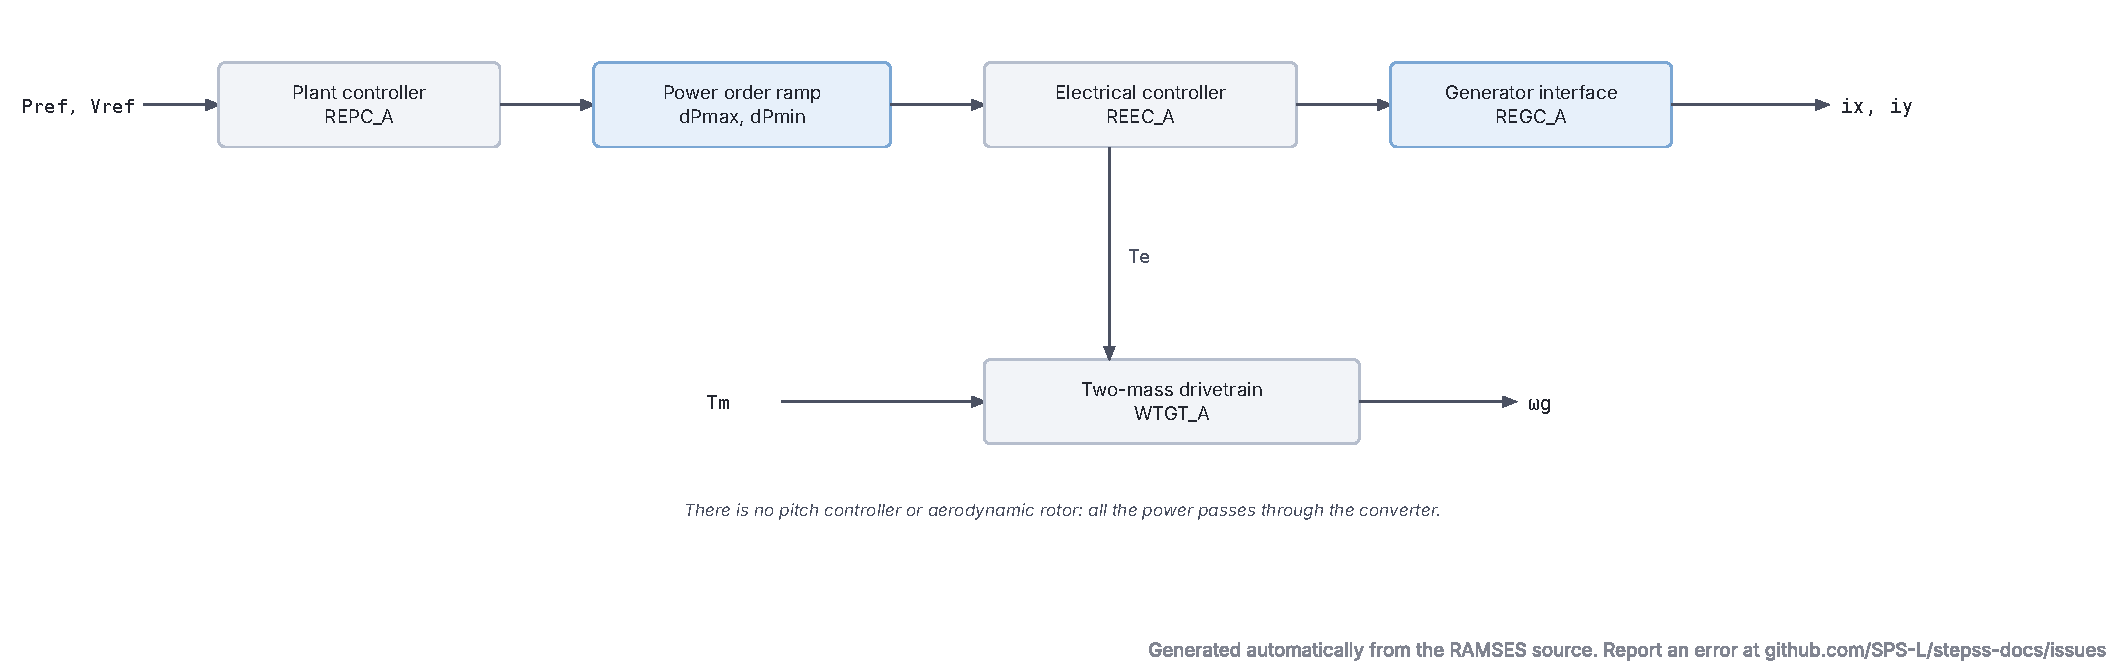
\includegraphics[width=0.98\linewidth]{figures/inj-wt4-light}
\caption{WT4 block diagram.}
\end{figure}

\subsection{Scientific Description}\label{model-inj-wecc:scientific-description-1}

\textbf{WTGT\_A, two-mass drivetrain.} The mechanical torque is the constant \(T_{mo} = P_{e0}/\omega_o\) and \(T_e = P_e/\omega_g\):

\[2H_t\frac{d\Delta\omega_t}{dt} = T_{mo} - K_{\mathrm{shaft}}\Delta\theta - D_{\mathrm{shaft}}(\Delta\omega_t - \Delta\omega_g)\]

\[2H_g\frac{d\Delta\omega_g}{dt} = K_{\mathrm{shaft}}\Delta\theta + D_{\mathrm{shaft}}(\Delta\omega_t - \Delta\omega_g) - T_e\]

\[\frac{d\Delta\theta}{dt} = \Delta\omega_t - \Delta\omega_g, \qquad \omega_g = \omega_o + \Delta\omega_g\]

As in WT3, the twist equation carries no base angular frequency, so \texttt{Kshaft} is per pu\ensuremath{\cdot}s of twist. Unlike WT3, the initial speed \(\omega_o\) is a data parameter.

\textbf{Coupling to the output.} The drivetrain reaches the network only through \texttt{PFlag}. With PFlag = 1 the power order is \(P_{\mathrm{ref}}\,\omega_g\), so a torsional oscillation of \(\omega_g\) modulates the active current. With PFlag = 0 the drivetrain is still computed but has no effect on the injection. The active power reference \(P_{\mathrm{ref}}\) is constant unless REPC\_A drives it (FreqFlag = 1), and is rate-limited by \texttt{dPmax} and \texttt{dPmin}.

\subsection{Parameters}\label{model-inj-wecc:parameters-1}

RAMSES applies \textbf{no default values}: a \texttt{WT4} record must carry exactly 103 values, and one with more or fewer is refused. Parameters 1--32 and 38--103 are listed in the parameter tables of \hyperref[model-inj-wecc:wt3-inj_wt3-type-3-wind-turbine-dfig]{WT3} under their \emph{WT4 \#}. The drivetrain block is specific to WT4:

\begin{small}\begin{longtable}[]{@{}
  >{\raggedright\arraybackslash}p{(\linewidth - 10\tabcolsep) * \real{0.1318}}
  >{\raggedright\arraybackslash}p{(\linewidth - 10\tabcolsep) * \real{0.1596}}
  >{\raggedright\arraybackslash}p{(\linewidth - 10\tabcolsep) * \real{0.3968}}
  >{\raggedright\arraybackslash}p{(\linewidth - 10\tabcolsep) * \real{0.1318}}
  >{\raggedright\arraybackslash}p{(\linewidth - 10\tabcolsep) * \real{0.1800}}
@{}}
\toprule\noalign{}
\begin{minipage}[b]{\linewidth}\raggedright
WT4 \#
\end{minipage} & \begin{minipage}[b]{\linewidth}\raggedright
Name
\end{minipage} & \begin{minipage}[b]{\linewidth}\raggedright
Description
\end{minipage} & \begin{minipage}[b]{\linewidth}\raggedright
Unit
\end{minipage} & \begin{minipage}[b]{\linewidth}\raggedright
Example
\end{minipage} \\
\midrule\noalign{}
\endhead
\bottomrule\noalign{}
\endlastfoot
33 & \texttt{Ht} & Turbine inertia & s & 3.395 \\
34 & \texttt{Hg} & Generator inertia & s & 0.962 \\
35 & \texttt{wo} & Initial generator speed, the reference of \(\Delta\omega_g\) & pu & 1 \\
36 & \texttt{Dshaft} & Shaft damping & pu/pu & 2.344 \\
37 & \texttt{Kshaft} & Shaft stiffness, per pu\ensuremath{\cdot}s of twist & pu & 1.387 \\
\end{longtable}\end{small}

The time-constant caution under the \hyperref[model-inj-wecc:wt3-inj_wt3-type-3-wind-turbine-dfig]{WT3 parameters} applies here too.

Twenty-eight further parameters are computed at initialization, the same as WT3 less the mechanical ones, plus \texttt{Tmo}, the constant mechanical torque.

\subsection{Observables}\label{model-inj-wecc:observables-1}

All quantities are in pu on \texttt{SNOM}.

\begin{small}\begin{longtable}[]{@{}
  >{\raggedright\arraybackslash}p{(\linewidth - 8\tabcolsep) * \real{0.1793}}
  >{\raggedright\arraybackslash}p{(\linewidth - 8\tabcolsep) * \real{0.3207}}
  >{\raggedright\arraybackslash}p{(\linewidth - 8\tabcolsep) * \real{0.1656}}
  >{\raggedright\arraybackslash}p{(\linewidth - 8\tabcolsep) * \real{0.3344}}
@{}}
\toprule\noalign{}
\begin{minipage}[b]{\linewidth}\raggedright
Name
\end{minipage} & \begin{minipage}[b]{\linewidth}\raggedright
Description
\end{minipage} & \begin{minipage}[b]{\linewidth}\raggedright
Name
\end{minipage} & \begin{minipage}[b]{\linewidth}\raggedright
Description
\end{minipage} \\
\midrule\noalign{}
\endhead
\bottomrule\noalign{}
\endlastfoot
\texttt{Pe}, \texttt{Qgen} & Terminal active and reactive power & \texttt{wg} & Generator speed \\
\texttt{vt} & Terminal voltage & \texttt{Te} & Electrical torque \\
\texttt{Freq} & Measured frequency & \texttt{Tmo} & Mechanical torque, constant \\
\texttt{vcon} & Compensated voltage & \texttt{Iqinj} & Dip reactive current injection \\
\texttt{Pbranch}, \texttt{Qbranch} & Powers at the compensated point & \texttt{Ipcmd}, \texttt{Iqcmd} & Current commands \\
\texttt{Pref}, \texttt{Qext} & Active and reactive references into REEC\_A & \texttt{Ipmax}, \texttt{Iqmax}, \texttt{Iqmin} & Current limits \\
\texttt{Plantpref}, \texttt{Qref}, \texttt{vref} & REPC\_A references, constant & \texttt{Ip}, \texttt{Iq} & Converter currents before the voltage management \\
\texttt{pfaref} & Initial power factor angle (rad), constant & \texttt{Ipf}, \texttt{Iqf} & Injected currents \\
& & \texttt{x59} & Low-voltage power logic limit on \(I_p\); reads \(10^9\) when inactive \\
\end{longtable}\end{small}

The initialization and its checks are those of \hyperref[model-inj-wecc:wt3-inj_wt3-type-3-wind-turbine-dfig]{WT3}.

\subsection{Usage Example}\label{model-inj-wecc:usage-example-1}

The WT3 example unit as a full converter: the same REPC\_A, REEC\_A, REGC\_A and PLL values, with the drivetrain block in place of WTGTRQ\_A, WTGPT\_A, WTGAR\_A and WTGT\_A.

\begin{Verbatim}
INJEC  WT4  WT4B03  B03
      # FP FQ P Q: share of the power-flow injection (FP, FQ) or initial power (P in MW, Q in Mvar)
      1.  1.  0.  0.
      # SNOM: Rating, base of every per-unit quantity in the model (MVA)
      1.667
      # Rc: Compensation resistance (pu)
      0
      # Xc: Compensation reactance (droop or line-drop) (pu)
      0
      # vcompFlag: 1: regulate lvertbar v_conrvert (line-drop compensation); 0: regulate v_t + K_c Q_branch (droop)
      0
      # Kc: Reactive droop gain (used when vcompFlag = 0) (pu/pu)
      0
      # Tfltr: Voltage and Q measurement filter; also the REGC_A voltage filter and the PLL input filter (s)
      0.02
      # RefFlag: 1: voltage control; 0: reactive power control
      1
      # dbd: Deadband on the V/Q error, symmetric, geq 0 (pu)
      0
      # emax: Upper limit on the V/Q error (pu)
      0.1
      # emin: Lower limit on the V/Q error (pu)
      -0.1
      # Kp: V/Q PI proportional gain (pu/pu)
      18
      # Ki: V/Q PI integral gain (pu/(pu*s))
      5
      # Qmax: Upper limit of the V/Q PI (pu)
      0.44
      # Qmin: Lower limit of the V/Q PI (pu)
      -0.44
      # Tft: Lead time constant (s)
      0
      # Tfv: Lag time constant; below 0.005 the lead-lag is bypassed (s)
      0.05
      # vfrz: Voltage below which the V/Q integrator is frozen (pu)
      0.7
      # Tp: Filter on P_branch and on the power-factor reference (s)
      0.05
      # fdbd1: Frequency deadband, lower edge, leq 0 (pu)
      -0.0006
      # fdbd2: Frequency deadband, upper edge, geq 0 (pu)
      0.0006
      # Ddn: Droop for over-frequency (pu/pu)
      20
      # Dup: Droop for under-frequency (pu/pu)
      0
      # femax: Upper limit on the power error (pu)
      999
      # femin: Lower limit on the power error (pu)
      -999
      # kpg: Power PI proportional gain (pu/pu)
      0.05
      # kig: Power PI integral gain (pu/(pu*s))
      0.1
      # Pmax: Upper limit of the power PI (pu)
      1
      # Pmin: Lower limit of the power PI (pu)
      0
      # Tlag: Lag on the plant power output (s)
      0.1
      # FreqFlag: 1: plant power loop sets P_refo; 0: P_refo held at its initial value
      0
      # Tmesf: Frequency measurement time constant, raised to 0.05 if smaller (s)
      0.02
      # QextFlag: 1: plant V/Q loop sets Q_ext; 0: Q_ext held at its initial value
      0
      # Ht: Turbine inertia (s)
      3.395
      # Hg: Generator inertia (s)
      0.962
      # wo: Initial generator speed, the reference of Deltaomega_g (pu)
      1
      # Dshaft: Shaft damping (pu/pu)
      2.344
      # Kshaft: Shaft stiffness, per pu*s of twist (pu)
      1.387
      # vdip: Voltage below which a dip is declared (pu)
      0.9
      # vup: Voltage above which a dip is declared (pu)
      1.1
      # Trv: Terminal voltage filter (s)
      0.02
      # vref0: Reference for the dip injection; used as given, so 0 is not replaced by the initial voltage (pu)
      1
      # vref1: Bias added to Q_r when vFlag = 0 (pu)
      1
      # dbd1: Dip injection deadband, lower edge, leq 0 (pu)
      -0.05
      # dbd2: Dip injection deadband, upper edge, geq 0 (pu)
      0.05
      # kqv: Dip reactive current gain (pu/pu)
      2
      # Iqh1: Upper limit of the dip injection (pu)
      1.05
      # Iql1: Lower limit of the dip injection (pu)
      -1.05
      # qmax: Upper limit of the reactive power reference (pu)
      0.44
      # qmin: Lower limit of the reactive power reference (pu)
      -0.44
      # vmax: Upper limit of V_ref and of the Q PI (pu)
      1.1
      # vmin: Lower limit of V_ref and of the Q PI (pu)
      0.9
      # kqp: Q PI proportional gain (pu/pu)
      0
      # kqi: Q PI integral gain (pu/(pu*s))
      0.1
      # kvp: V PI proportional gain (pu/pu)
      0
      # kvi: V PI integral gain (pu/(pu*s))
      40
      # Tiq: Reactive current lag (QFlag = 0) (s)
      0.02
      # vq1: VDL1, voltage of point 1 (pu)
      0.2
      # Iq1: VDL1, reactive current limit at point 1 (pu)
      1
      # vq2: VDL1, point 2 (pu)
      0.4
      # Iq2:  (pu)
      1
      # vq3: VDL1, point 3 (pu)
      0.8
      # Iq3:  (pu)
      1
      # vq4: VDL1, point 4 (pu)
      1
      # Iq4:  (pu)
      1
      # vp1: VDL2, voltage of point 1 (pu)
      0.2
      # Ip1: VDL2, active current limit at point 1 (pu)
      1
      # vp2: VDL2, point 2 (pu)
      0.4
      # Ip2:  (pu)
      1
      # vp3: VDL2, point 3 (pu)
      0.8
      # Ip3:  (pu)
      1
      # vp4: VDL2, point 4 (pu)
      1
      # Ip4:  (pu)
      1
      # dPmax: Upper rate limit of P_ref (pu/s)
      999
      # dPmin: Lower rate limit of P_ref (pu/s)
      -999
      # pmax: Upper limit of the power order Pord (pu)
      1
      # pmin: Lower limit of the power order Pord (pu)
      0
      # Tpord: Power order lag (s)
      0.02
      # Imax: Converter current limit (pu)
      1.11
      # Thld: Post-dip hold of the reactive injection; its sign selects the mode (s)
      0
      # Thld2: Post-dip hold of I_pmax (s)
      0
      # Iqfrz: Reactive injection held after a dip when Thld > 0 (pu)
      0
      # PFFlag: 1: constant power factor; 0: reactive power reference Q_ext
      0
      # vFlag: 1: V_ref from the Q PI; 0: V_ref = Q_r + v_ref1
      0
      # QFlag: 1: reactive current from the voltage PI; 0: from Q_r/v_t
      0
      # PQFlag: 1: active current priority; 0: reactive current priority
      0
      # PFlag: 1: power order is P_ref,omega_g; 0: power order is P_ref
      1
      # Iqrmax: Reactive current rate limit, used when Q_0 > 0 (pu/s)
      999
      # Iqrmin: Reactive current rate limit, used when Q_0 < 0 (pu/s)
      -999
      # Tg: Converter current lag (s)
      0.02
      # vtmax: High-voltage threshold (WECC Volim) (pu)
      1.2
      # accel: High-voltage reactive current gain (WECC Khv) (pu/pu)
      0.7
      # QMIN: Lower limit of the converter reactive output after the high-voltage reduction (pu)
      -1.3
      # lvpnt0: Active current is zero below this voltage (pu)
      0.4
      # lvpnt1: Active current is unreduced above this voltage (pu)
      0.8
      # Brkpt: Low-voltage power logic breakpoint (pu)
      0.9
      # zerox: Low-voltage power logic zero crossing (pu)
      0.4
      # Lvpl1: Low-voltage power logic limit at Brkpt (pu)
      1.22
      # Lvplsw: 1: low-voltage power logic on; 0: off
      0
      # rrpwr: Active current rise rate limit (pu/s)
      10
      # vPLL: Voltage below which the PLL angle is frozen (pu)
      0.2
      # kpPLL: PLL proportional gain (rad/s/pu)
      3
      # kiPLL: PLL integral gain (rad/s^2/pu)
      30
      # wrefPLL: PLL frequency offset; cancels, no effect on the response
      1
;
\end{Verbatim}

\begin{docsnote}{Note}

With this record, as with the WT3 one, RAMSES reports \texttt{INJECTORS\ NOT\ IN\ STEADY\ STATE} at initialization. The residuals are on the Q and V PI controllers of REEC\_A, which \texttt{QFlag} = 0 takes out of the loop, and whose initial values the model does not yet set consistently; one of their limiters also toggles during the first time step.

\end{docsnote}

\begin{center}\rule{0.5\linewidth}{0.5pt}\end{center}

\section{\texorpdfstring{BESS (\texttt{inj\_BESS}): Battery Energy Storage System}{BESS (inj\_BESS): Battery Energy Storage System}}\label{model-inj-wecc:bess-inj_bess-battery-energy-storage-system}

The data-file model name is \texttt{BESS} (or \texttt{inj\_BESS}).

\subsection{Description}\label{model-inj-wecc:description-2}

A comprehensive BESS model implementing the full WECC framework (REPC\_A + REEC\_C + REGC\_A) plus battery state of charge (SOC) tracking. The model supports both grid-following operation (bidirectional active power dispatch) and reactive power / voltage regulation. It is built on the same REPC\_A plant controller as the wind turbine models, and uses the REEC\_C converter electrical controller which handles a piecewise-linear \(I_q\)-vs-\(V\) and \(I_p\)-vs-\(V\) characteristic for fault ride-through.

The battery SOC evolves through integration of injected power:

\[\frac{d\mathrm{SOC}}{dt} = -\frac{P_{\mathrm{bess}}}{C_{\mathrm{bat}} \cdot S_{\mathrm{nom}}}\]

with hard clamps at \texttt{SOCmin} and \texttt{SOCmax} that modify the active power limits \texttt{Pmax}/\texttt{Pmin} dynamically:

\[P_{\max} = \begin{cases} 0 & \mathrm{SOC} \ge \mathrm{SOC}_{\max}\\ P_{\max,\mathrm{rated}} & \text{otherwise}\end{cases}\]

\[P_{\min} = \begin{cases} 0 & \mathrm{SOC} \le \mathrm{SOC}_{\min}\\ P_{\min,\mathrm{rated}} & \text{otherwise}\end{cases}\]

\begin{figure}[htbp]
\centering
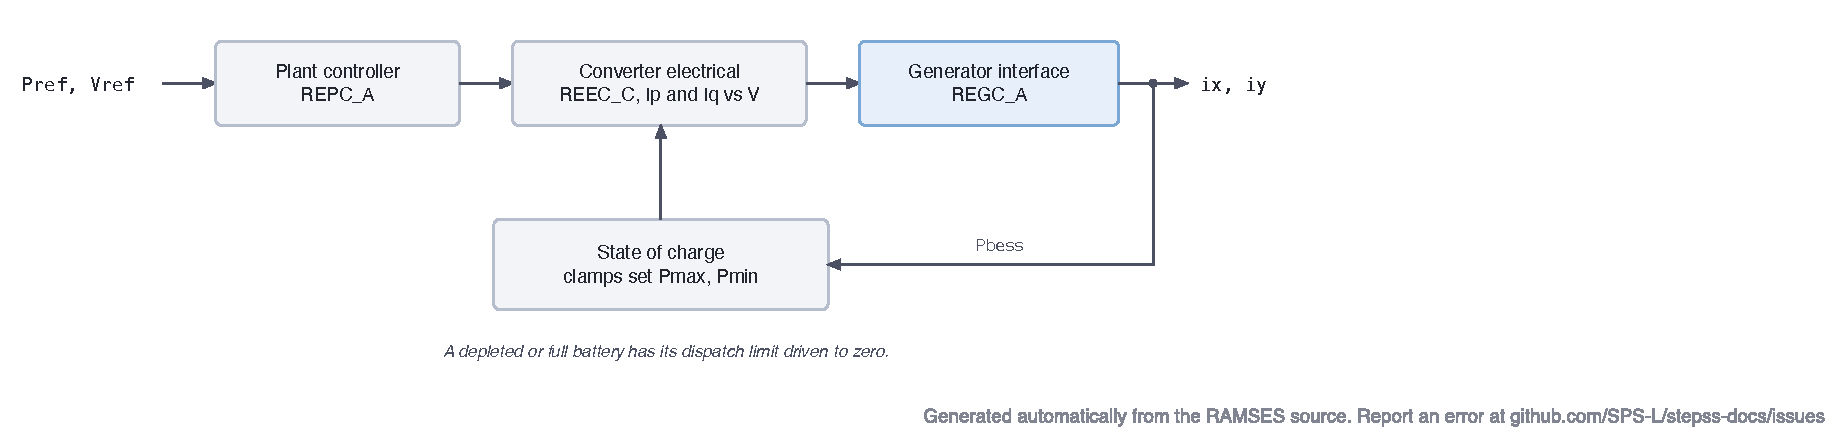
\includegraphics[width=0.98\linewidth]{figures/inj-bess-light}
\caption{Battery energy storage block diagram.}
\end{figure}

\subsection{Parameters (key parameters)}\label{model-inj-wecc:parameters-key-parameters}

\begin{small}\begin{longtable}[]{@{}
  >{\raggedright\arraybackslash}p{(\linewidth - 10\tabcolsep) * \real{0.1349}}
  >{\raggedright\arraybackslash}p{(\linewidth - 10\tabcolsep) * \real{0.1752}}
  >{\raggedright\arraybackslash}p{(\linewidth - 10\tabcolsep) * \real{0.1660}}
  >{\raggedright\arraybackslash}p{(\linewidth - 10\tabcolsep) * \real{0.3870}}
  >{\raggedright\arraybackslash}p{(\linewidth - 10\tabcolsep) * \real{0.1368}}
@{}}
\toprule\noalign{}
\begin{minipage}[b]{\linewidth}\raggedright
\#
\end{minipage} & \begin{minipage}[b]{\linewidth}\raggedright
Name
\end{minipage} & \begin{minipage}[b]{\linewidth}\raggedright
Sub-model
\end{minipage} & \begin{minipage}[b]{\linewidth}\raggedright
Description
\end{minipage} & \begin{minipage}[b]{\linewidth}\raggedright
Unit
\end{minipage} \\
\midrule\noalign{}
\endhead
\bottomrule\noalign{}
\endlastfoot
1 & \texttt{SNOM} & & Nominal power & MW \\
2--32 & & REPC\_A & Plant controller (same as WT3/WT4) & various \\
33--76 & & REEC\_C & Electrical controller with piecewise \(I_q(V)\), \(I_p(V)\) & various \\
68 & \texttt{CapBat} & BESS & Battery energy capacity & MWh \\
69 & \texttt{SOCini} & BESS & Initial state of charge & pu \\
70 & \texttt{SOCmax} & BESS & Maximum SOC limit & pu \\
71 & \texttt{SOCmin} & BESS & Minimum SOC limit & pu \\
72--73 & \texttt{dPmax}, \texttt{dPmin} & BESS & Active power ramp rate limits & pu/s \\
74--75 & \texttt{pmax}, \texttt{pmin} & REEC\_C & Active current limits (pu on SNOM) & pu \\
76 & \texttt{Tpord} & REEC\_C & Active power order time constant & s \\
\end{longtable}\end{small}

Full parameter listing has approximately 125 parameters; refer to a working example data file for the complete ordering.

\subsection{State Variables}\label{model-inj-wecc:state-variables}

The BESS model uses over 40 internal states reflecting the three sub-models. Key states include:

\begin{small}\begin{longtable}[]{@{}ll@{}}
\toprule\noalign{}
Variable & Description \\
\midrule\noalign{}
\endhead
\bottomrule\noalign{}
\endlastfoot
\texttt{SOC} & State of charge \\
\texttt{Pref} & Active power reference \\
\texttt{Qext} & Reactive power reference from REPC\_A \\
\texttt{Ip}, \texttt{Iq} & Active/reactive current outputs \\
\texttt{PLLPhaseAngle} & PLL phase angle \\
\texttt{Pgen}, \texttt{Qgen} & Generated powers \\
\end{longtable}\end{small}

\subsection{Usage Example}\label{model-inj-wecc:usage-example-2}

\begin{Verbatim}
INJEC  BESS  BESS1  BUS_ST
      # FP FQ P Q: share of the power-flow injection (FP, FQ) or initial power (P in MW, Q in Mvar)
      1.  1.  0.  0.
      # SNOM: Rating, base of every per-unit quantity in the model (MVA)
      100.
      # Rc: Compensation resistance (pu)
      0
      # Xc: Compensation reactance (droop or line-drop) (pu)
      0
      # vcompFlag: 1: regulate lvertbar v_conrvert (line-drop compensation); 0: regulate v_t + K_c Q_branch (droop)
      0
      # Kc: Reactive droop gain (used when vcompFlag = 0) (pu/pu)
      0
      # Tfltr: Voltage and Q measurement filter; also the REGC_A voltage filter and the PLL input filter (s)
      0.02
      # RefFlag: 1: voltage control; 0: reactive power control
      1
      # dbd: Deadband on the V/Q error, symmetric, geq 0 (pu)
      0
      # emax: Upper limit on the V/Q error (pu)
      0.1
      # emin: Lower limit on the V/Q error (pu)
      -0.1
      # Kp: V/Q PI proportional gain (pu/pu)
      18
      # Ki: V/Q PI integral gain (pu/(pu*s))
      5
      # Qmax: Upper limit of the V/Q PI (pu)
      0.44
      # Qmin: Lower limit of the V/Q PI (pu)
      -0.44
      # Tft: Lead time constant (s)
      0
      # Tfv: Lag time constant; below 0.005 the lead-lag is bypassed (s)
      0.05
      # vfrz: Voltage below which the V/Q integrator is frozen (pu)
      0.7
      # Tp: Filter on P_branch and on the power-factor reference (s)
      0.05
      # fdbd1: Frequency deadband, lower edge, leq 0 (pu)
      -0.0006
      # fdbd2: Frequency deadband, upper edge, geq 0 (pu)
      0.0006
      # Ddn: Droop for over-frequency (pu/pu)
      20
      # Dup: Droop for under-frequency (pu/pu)
      0
      # femax: Upper limit on the power error (pu)
      999
      # femin: Lower limit on the power error (pu)
      -999
      # kpg: Power PI proportional gain (pu/pu)
      0.05
      # kig: Power PI integral gain (pu/(pu*s))
      0.1
      # Pmax: Upper limit of the power PI (pu)
      1
      # Pmin: Lower limit of the power PI (pu)
      -1
      # Tlag: Lag on the plant power output (s)
      0.1
      # FreqFlag: 1: plant power loop sets P_refo; 0: P_refo held at its initial value
      0
      # Tmesf: Frequency measurement time constant, raised to 0.05 if smaller (s)
      0.02
      # QextFlag: 1: plant V/Q loop sets Q_ext; 0: Q_ext held at its initial value
      0
      # vdip: Voltage below which a dip is declared (pu)
      0.9
      # vup: Voltage above which a dip is declared (pu)
      1.1
      # Trv: Terminal voltage filter (s)
      0.02
      # vref0: Reference for the dip injection; used as given, so 0 is not replaced by the initial voltage (pu)
      1
      # dbd1: Dip injection deadband, lower edge, leq 0 (pu)
      -0.05
      # dbd2: Dip injection deadband, upper edge, geq 0 (pu)
      0.05
      # kqv: Dip reactive current gain (pu/pu)
      2
      # Iqh1: Upper limit of the dip injection (pu)
      1.05
      # Iql1: Lower limit of the dip injection (pu)
      -1.05
      # qmax: Upper limit of the reactive power reference (pu)
      0.44
      # qmin: Lower limit of the reactive power reference (pu)
      -0.44
      # vmax: Upper limit of V_ref and of the Q PI (pu)
      1.1
      # vmin: Lower limit of V_ref and of the Q PI (pu)
      0.9
      # kqp: Q PI proportional gain (pu/pu)
      0
      # kqi: Q PI integral gain (pu/(pu*s))
      0.1
      # kvp: V PI proportional gain (pu/pu)
      0
      # kvi: V PI integral gain (pu/(pu*s))
      40
      # Tiq: Reactive current lag (QFlag = 0) (s)
      0.02
      # vq1: VDL1, voltage of point 1 (pu)
      0.2
      # Iq1: VDL1, reactive current limit at point 1 (pu)
      1
      # vq2: VDL1, point 2 (pu)
      0.4
      # Iq2:  (pu)
      1
      # vq3: VDL1, point 3 (pu)
      0.8
      # Iq3:  (pu)
      1
      # vq4: VDL1, point 4 (pu)
      1
      # Iq4:  (pu)
      1
      # vp1: VDL2, voltage of point 1 (pu)
      0.2
      # Ip1: VDL2, active current limit at point 1 (pu)
      1
      # vp2: VDL2, point 2 (pu)
      0.4
      # Ip2:  (pu)
      1
      # vp3: VDL2, point 3 (pu)
      0.8
      # Ip3:  (pu)
      1
      # vp4: VDL2, point 4 (pu)
      1
      # Ip4:  (pu)
      1
      # Paux: Constant added to the active current command after dividing Pord by voltage (Ipcmd = Pord/V + Paux), on SNOM base (pu)
      0.
      # CapBat: Battery energy capacity (MWh)
      100.
      # SOCini: Initial state of charge as a fraction of CapBat; must lie strictly between SOCmin and SOCmax (pu)
      0.5
      # SOCmax: Upper SOC limit; at it the battery is full and charging current is blocked (Ipmin = 0) (pu)
      0.9
      # SOCmin: Lower SOC limit; at it the battery is empty and discharging current is blocked (Ipmax = 0) (pu)
      0.1
      # dPmax: Upper rate limit of P_ref (pu/s)
      999
      # dPmin: Lower rate limit of P_ref (pu/s)
      -999
      # pmax: Upper limit of the power order Pord (pu)
      1
      # pmin: Lower limit of the power order Pord (pu)
      -1
      # Tpord: Active power order time constant (s)
      0.02
      # Imax: Converter current limit (pu)
      1.11
      # PFFlag: 1: constant power factor; 0: reactive power reference Q_ext
      0
      # vFlag: 1: V_ref from the Q PI; 0: V_ref = Q_r + v_ref1
      0
      # QFlag: 1: reactive current from the voltage PI; 0: from Q_r/v_t
      0
      # PQFlag: 1: active current priority; 0: reactive current priority
      0
      # Iqrmax: Reactive current rate limit, used when Q_0 > 0 (pu/s)
      999
      # Iqrmin: Reactive current rate limit, used when Q_0 < 0 (pu/s)
      -999
      # Tg: Converter current lag (s)
      0.02
      # vtmax: High-voltage threshold (WECC Volim) (pu)
      1.2
      # accel: High-voltage reactive current gain (WECC Khv) (pu/pu)
      0.7
      # QMIN: Lower limit of the converter reactive output after the high-voltage reduction (pu)
      -1.3
      # lvpnt0: Active current is zero below this voltage (pu)
      0.4
      # lvpnt1: Active current is unreduced above this voltage (pu)
      0.8
      # Brkpt: Low-voltage power logic breakpoint (pu)
      0.9
      # zerox: Low-voltage power logic zero crossing (pu)
      0.4
      # Lvpl1: Low-voltage power logic limit at Brkpt (pu)
      1.22
      # Lvplsw: 1: low-voltage power logic on; 0: off
      0
      # rrpwr: Active current rise rate limit (pu/s)
      10
      # vPLL: Voltage below which the PLL angle is frozen (pu)
      0.2
      # kpPLL: PLL proportional gain (rad/s/pu)
      3
      # kiPLL: PLL integral gain (rad/s^2/pu)
      30
      # wrefPLL: PLL frequency offset; cancels, no effect on the response
      1
;
\end{Verbatim}
